\documentclass{article}
\usepackage[UTF8,scheme=plain,fontset=fandol]{ctex}
% If your build breaks (sometimes temporarily if a hyperlink spans a page)
% please comment out the following usepackage line and replace
% \usepackage{icml2025} with \usepackage[nohyperref]{icml2025} above.
\usepackage{hyperref}

\usepackage{graphicx}
\usepackage{amsmath}
\usepackage{amssymb}
\usepackage{subfigure}
\usepackage{booktabs}

\usepackage{url}            % simple URL typesetting
\usepackage{amsfonts}       % blackboard math symbols
\usepackage{nicefrac}       % compact symbols for 1/2, etc.
\usepackage{microtype}      % microtypography

\usepackage{makecell}
\usepackage{amsthm}
\usepackage{mathtools}
\usepackage{bm}
\usepackage[table,xcdraw]{xcolor}
\usepackage{multicol}
\usepackage{colortbl}
\usepackage{multirow}
% \usepackage[normalem]{ulem}
% \useunder{\uline}{\ul}{}
\usepackage{enumitem}
%\usepackage{stfloats}
% \usepackage{threeparttable}  
\usepackage{bbding}
\usepackage{color}
% \usepackage{balance}
\usepackage{dsfont}
\usepackage{algorithm}
\usepackage{listings}
\usepackage{natbib}
\usepackage[capitalize,noabbrev]{cleveref}

\newcommand{\black}[1]{\textcolor{black}{#1}}
% Copy from MoCo
%----------------------------------------------------------
% this is for adding footnote after algorithm
\usepackage{etoolbox}
\makeatletter
\AfterEndEnvironment{algorithm}{\let\@algcomment\relax}
\AtEndEnvironment{algorithm}{\kern2pt\hrule\relax\vskip3pt\@algcomment}
\let\@algcomment\relax
\newcommand\algcomment[1]{\def\@algcomment{\footnotesize#1}}
\renewcommand\fs@ruled{\def\@fs@cfont{\bfseries}\let\@fs@capt\floatc@ruled
  \def\@fs@pre{\hrule height.8pt depth0pt \kern2pt}%
  \def\@fs@post{}%
  \def\@fs@mid{\kern2pt\hrule\kern2pt}%
  \let\@fs@iftopcapt\iftrue}
\makeatother


%%%%%%%%%%%%%%%%%%%%%%%%%%%%%%%%
% THEOREMS
%%%%%%%%%%%%%%%%%%%%%%%%%%%%%%%%
\theoremstyle{plain}
\newtheorem{theorem}{Theorem}[section]
\newtheorem{proposition}[theorem]{Proposition}
\newtheorem{lemma}[theorem]{Lemma}
\newtheorem{corollary}[theorem]{Corollary}
\theoremstyle{definition}
\newtheorem{definition}[theorem]{Definition}
\newtheorem{assumption}[theorem]{Assumption}
\theoremstyle{remark}
\newtheorem{remark}[theorem]{Remark}

% Todonotes is useful during development; simply uncomment the next line
%    and comment out the line below the next line to turn off comments
%\usepackage[disable,textsize=tiny]{todonotes}
\usepackage[textsize=tiny]{todonotes}


\usepackage[table]{xcolor}



\definecolor{ourscolor}{HTML}{E8E8FF}

\definecolor{basegray}{HTML}{F5F5F5}  % F5F5F5 是一个非常柔和、不刺眼的灰色


\definecolor{ForestGreen}{RGB}{34,139,34}

\newcommand{\dui}{\textcolor{teal}{\CheckmarkBold}}
\newcommand{\cuo}{\textcolor{purple}{\XSolidBrush}}
\newcommand{\aka}{\emph{aka}~}
\renewcommand{\paragraph}[1]{\medskip\noindent\textbf{#1.~}}

\newcommand{\xiaok}[1]{\left(#1\right)}
\newcommand{\zhongk}[1]{\left[#1\right]}
\newcommand{\dak}[1]{\left\{#1\right\}}
\newcommand{\jiaok}[1]{\left<#1\right>}
\newcommand{\shuk}[1]{\left\lVert#1\right\rVert}
\newcommand{\shuks}[1]{\left\lVert#1\right\rVert^2}
\newcommand{\shangk}[1]{\left\lceil #1 \right\rceil}
\newcommand{\xiak}[1]{\left\lfloor #1 \right\rfloor}

\newcommand{\argmax}[1]{{\mathop{\arg\mathrm{max}}_{#1}\,}}
\newcommand{\argmin}[1]{{\mathop{\arg\mathrm{min}}_{#1}\,}}
\newcommand{\pfrac}[2]{\frac{\partial #1}{\partial #2}}
\newcommand{\prob}[2]{p\xiaok{#1 \mid #2}}

\newcommand{\T}{\top}
\newcommand{\dif}{\mathop{}\!\mathrm{d}}
\newcommand{\biset}[1]{\{0,1\}^{#1}}
\newcommand{\ReLU}{\mathrm{ReLU}}
\newcommand{\relu}{\mathrm{ReLU}}
\newcommand{\sign}{\mathrm{sign}}
\newcommand\softmax{\mathrm{softmax}}
\newcommand\KL{D_{\mathrm{KL}}}
\newcommand\Var{\mathrm{Var}}
\newcommand\Cov{\mathrm{Cov}}
\newcommand{\Tr}{\mathrm{Tr}}
\newcommand{\tr}{\mathrm{tr}}
\newcommand{\dist}{\mathrm{dist}}
\newcommand{\concat}{\mathrm{concat}}
\newcommand{\mean}{\mathrm{mean}}
\newcommand{\diag}{\mathrm{diag}}
\newcommand{\cov}{\mathrm{cov}}

\newcommand{\range}[1]{{0,1,\cdots,#1}} % 0, 1, ..., N
\newcommand{\Range}[1]{{1,2,\cdots,#1}} % 1, 2, ..., N
\newcommand{\opseq}[3]{{#1_1 #3 #1_2 #3 \cdots #3 #1_{#2}}}
\newcommand{\seq}[2]{\opseq{#1}{#2}{,}}
\newcommand{\xseq}[2]{\opseq{#1}{#2}{\times}}

\newcommand{\bma}{\bm{a}}
\newcommand{\bmb}{\bm{b}}
\newcommand{\bmc}{\bm{c}}
\newcommand{\bmd}{\bm{d}}
\newcommand{\bme}{\bm{e}}
\newcommand{\bmf}{\bm{f}}
\newcommand{\bmg}{\bm{g}}
\newcommand{\bmh}{\bm{h}}
\newcommand{\bmi}{\bm{i}}
\newcommand{\bmj}{\bm{j}}
\newcommand{\bmk}{\bm{k}}
\newcommand{\bml}{\bm{l}}
\newcommand{\bmm}{\bm{m}}
\newcommand{\bmn}{\bm{n}}
\newcommand{\bmo}{\bm{o}}
\newcommand{\bmp}{\bm{p}}
\newcommand{\bmq}{\bm{q}}
\newcommand{\bmr}{\bm{r}}
\newcommand{\bms}{\bm{s}}
\newcommand{\bmt}{\bm{t}}
\newcommand{\bmu}{\bm{u}}
\newcommand{\bmv}{\bm{v}}
\newcommand{\bmw}{\bm{w}}
\newcommand{\bmx}{\bm{x}}
\newcommand{\bmy}{\bm{y}}
\newcommand{\bmz}{\bm{z}}
\newcommand{\bmzero}{\bm{0}}
\newcommand{\bmone}{\bm{1}}
\newcommand{\bmalpha}{\bm{\alpha}}
\newcommand{\bmbeta}{\bm{\beta}}
\newcommand{\bmgamma}{\bm{\gamma}}
\newcommand{\bmdelta}{\bm{\delta}}
\newcommand{\bmepsilon}{\bm{\epsilon}}
\newcommand{\bmtheta}{\bm{\theta}}
\newcommand{\bmiota}{\bm{\iota}}
\newcommand{\bmkappa}{\bm{\kappa}}
\newcommand{\bmlambda}{\bm{\lambda}}
\newcommand{\bmmu}{\bm{\mu}}
\newcommand{\bmnu}{\bm{\nu}}
\newcommand{\bmxi}{\bm{\xi}}
\newcommand{\bmpi}{\bm{\pi}}
\newcommand{\bmrho}{\bm{\rho}}
\newcommand{\bmsigma}{\bm{\sigma}}
\newcommand{\bmtau}{\bm{\tau}}
\newcommand{\bmupsilon}{\bm{\upsilon}}
\newcommand{\bmphi}{\bm{\phi}}
\newcommand{\bmchi}{\bm{\chi}}
\newcommand{\bmpsi}{\bm{\psi}}
\newcommand{\bmomega}{\bm{\omega}}
\newcommand{\bmA}{\bm{A}}
\newcommand{\bmB}{\bm{B}}
\newcommand{\bmC}{\bm{C}}
\newcommand{\bmD}{\bm{D}}
\newcommand{\bmE}{\bm{E}}
\newcommand{\bmF}{\bm{F}}
\newcommand{\bmG}{\bm{G}}
\newcommand{\bmH}{\bm{H}}
\newcommand{\bmI}{\bm{I}}
\newcommand{\bmJ}{\bm{J}}
\newcommand{\bmK}{\bm{K}}
\newcommand{\bmL}{\bm{L}}
\newcommand{\bmM}{\bm{M}}
\newcommand{\bmN}{\bm{N}}
\newcommand{\bmO}{\bm{O}}
\newcommand{\bmP}{\bm{P}}
\newcommand{\bmQ}{\bm{Q}}
\newcommand{\bmR}{\bm{R}}
\newcommand{\bmS}{\bm{S}}
\newcommand{\bmT}{\bm{T}}
\newcommand{\bmU}{\bm{U}}
\newcommand{\bmV}{\bm{V}}
\newcommand{\bmW}{\bm{W}}
\newcommand{\bmX}{\bm{X}}
\newcommand{\bmY}{\bm{Y}}
\newcommand{\bmZ}{\bm{Z}}
\newcommand{\bmGamma}{\bm{\Gamma}}
\newcommand{\bmDelta}{\bm{\Delta}}
\newcommand{\bmTheta}{\bm{\Theta}}
\newcommand{\bmLambda}{\bm{\Lambda}}
\newcommand{\bmXi}{\bm{\Xi}}
\newcommand{\bmPi}{\bm{\Pi}}
\newcommand{\bmSigma}{\bm{\Sigma}}
\newcommand{\bmUpsilon}{\bm{\Upsilon}}
\newcommand{\bmPhi}{\bm{\Phi}}
\newcommand{\bmPsi}{\bm{\Psi}}
\newcommand{\bmOmega}{\bm{\Omega}}

\newcommand{\calA}{\mathcal{A}}
\newcommand{\calB}{\mathcal{B}}
\newcommand{\calC}{\mathcal{C}}
\newcommand{\calD}{\mathcal{D}}
\newcommand{\calE}{\mathcal{E}}
\newcommand{\calF}{\mathcal{F}}
\newcommand{\calG}{\mathcal{G}}
\newcommand{\calH}{\mathcal{H}}
\newcommand{\calI}{\mathcal{I}}
\newcommand{\calJ}{\mathcal{J}}
\newcommand{\calK}{\mathcal{K}}
\newcommand{\calL}{\mathcal{L}}
\newcommand{\calM}{\mathcal{M}}
\newcommand{\calN}{\mathcal{N}}
\newcommand{\calO}{\mathcal{O}}
\newcommand{\calP}{\mathcal{P}}
\newcommand{\calQ}{\mathcal{Q}}
\newcommand{\calR}{\mathcal{R}}
\newcommand{\calS}{\mathcal{S}}
\newcommand{\calT}{\mathcal{T}}
\newcommand{\calU}{\mathcal{U}}
\newcommand{\calV}{\mathcal{V}}
\newcommand{\calW}{\mathcal{W}}
\newcommand{\calX}{\mathcal{X}}
\newcommand{\calY}{\mathcal{Y}}
\newcommand{\calZ}{\mathcal{Z}}

\newcommand{\bbC}{\mathbb{C}}
\newcommand{\bbE}{\mathbb{E}}
\newcommand{\bbI}{\mathbb{I}}
\newcommand{\bbN}{\mathbb{N}}
\newcommand{\bbQ}{\mathbb{Q}}
\newcommand{\bbR}{\mathbb{R}}
\newcommand{\bbZ}{\mathbb{Z}}

\newcommand{\tabincell}[2]{\begin{tabular}{@{}#1@{}}#2\end{tabular}}

\definecolor{medievalred}{RGB}{120,30,40}

\newcommand{\modelname}{%
  \scalebox{1.1}{%
    {\itshape
    \textbf{%
      \textcolor{medievalred}{Holmes}%
    }}%
  }%
}


\usepackage[accepted]{icml2026}
\setmainfont{Latin Modern Roman}
\setsansfont{Latin Modern Sans}
\setmonofont{Latin Modern Mono}
\setCJKmainfont{FandolSong-Regular.otf}[
  BoldFont=FandolSong-Bold.otf,ItalicFont=FandolKai-Regular.otf,
  BoldItalicFont=FandolKai-Regular.otf]
\patchcmd{\abstract}{Abstract}{摘要}{}{}
\renewcommand{\refname}{参考文献}

\icmltitlerunning{Holmes}

\begin{document}

\twocolumn[
\icmltitle{重新审视不确定性：部分相关视频检索中的证据学习}



\begin{icmlauthorlist}
\icmlauthor{Jun Li}{thusz,pcl}
\icmlauthor{Peifeng Lai}{hitsz}
\icmlauthor{Xuhang Lou}{hitsz}
\icmlauthor{Jinpeng Wang}{hitsz}
\icmlauthor{Yuting Wang}{}\\
\icmlauthor{Ke Chen}{pcl}
\icmlauthor{Yaowei Wang}{hitsz,pcl}
\icmlauthor{Shu-tao Xia}{thusz,pcl}
\end{icmlauthorlist}

\icmlaffiliation{thusz}{Tsinghua Shenzhen International Graduate School, Tsinghua University, Shenzhen, China}
\icmlaffiliation{hitsz}{Harbin Institute of Technology, Shenzhen, China}
\icmlaffiliation{pcl}{Peng Cheng Laboratory, Shenzhen, China}


\icmlcorrespondingauthor{Jinpeng Wang}{wangjp26@gmail.com}

% the "keywords" metadata in the PDF but will not be shown in the document
\icmlkeywords{机器学习, ICML}

\vskip 0.3in
]

\printAffiliationsAndNotice{}  % leave blank if no need to mention equal contribution
% \printAffiliationsAndNotice{\icmlEqualContribution} % otherwise use the standard text.

\begin{abstract}
部分相关视频检索旨在根据只描述部分内容的文本查询，找出未经剪辑的视频。然而，简短查询与丰富视频内容之间固有的不对称，必然给检索过程带来\emph{不确定性}。在这一场景中，含糊的查询往往造成视频间\emph{语义歧义}；与此同时，视频内的\emph{稀疏时序监督}无法提供充分的匹配证据，进一步加剧了这一问题。

为此，我们提出分层证据学习框架 \modelname{}，通过汇聚不同粒度的跨模态证据，显式量化并建模不确定性。在\textbf{视频间}层面，我们将相似度分数视为证据支持，并以 Dirichlet 分布建模。基于所提出的三项判别原则，我们对查询进行细粒度识别，进而开展查询自适应的校准学习。在\textbf{视频内}层面，为积累更密集的证据，我们采用带自适应回收槽的灵活最优传输，构建查询与片段之间的软对齐，从而缓解时序监督稀疏，并抑制虚假局部响应。大量实验表明，\modelname{} 优于当前先进方法。代码发布于 \href{https://github.com/lijun2005/ICML26-Holmes}{ICML26-Holmes}。
\end{abstract}
% Gemini生成
\section{引言}
\label{sec:intro}
\begin{figure*}[t]
    \centering
    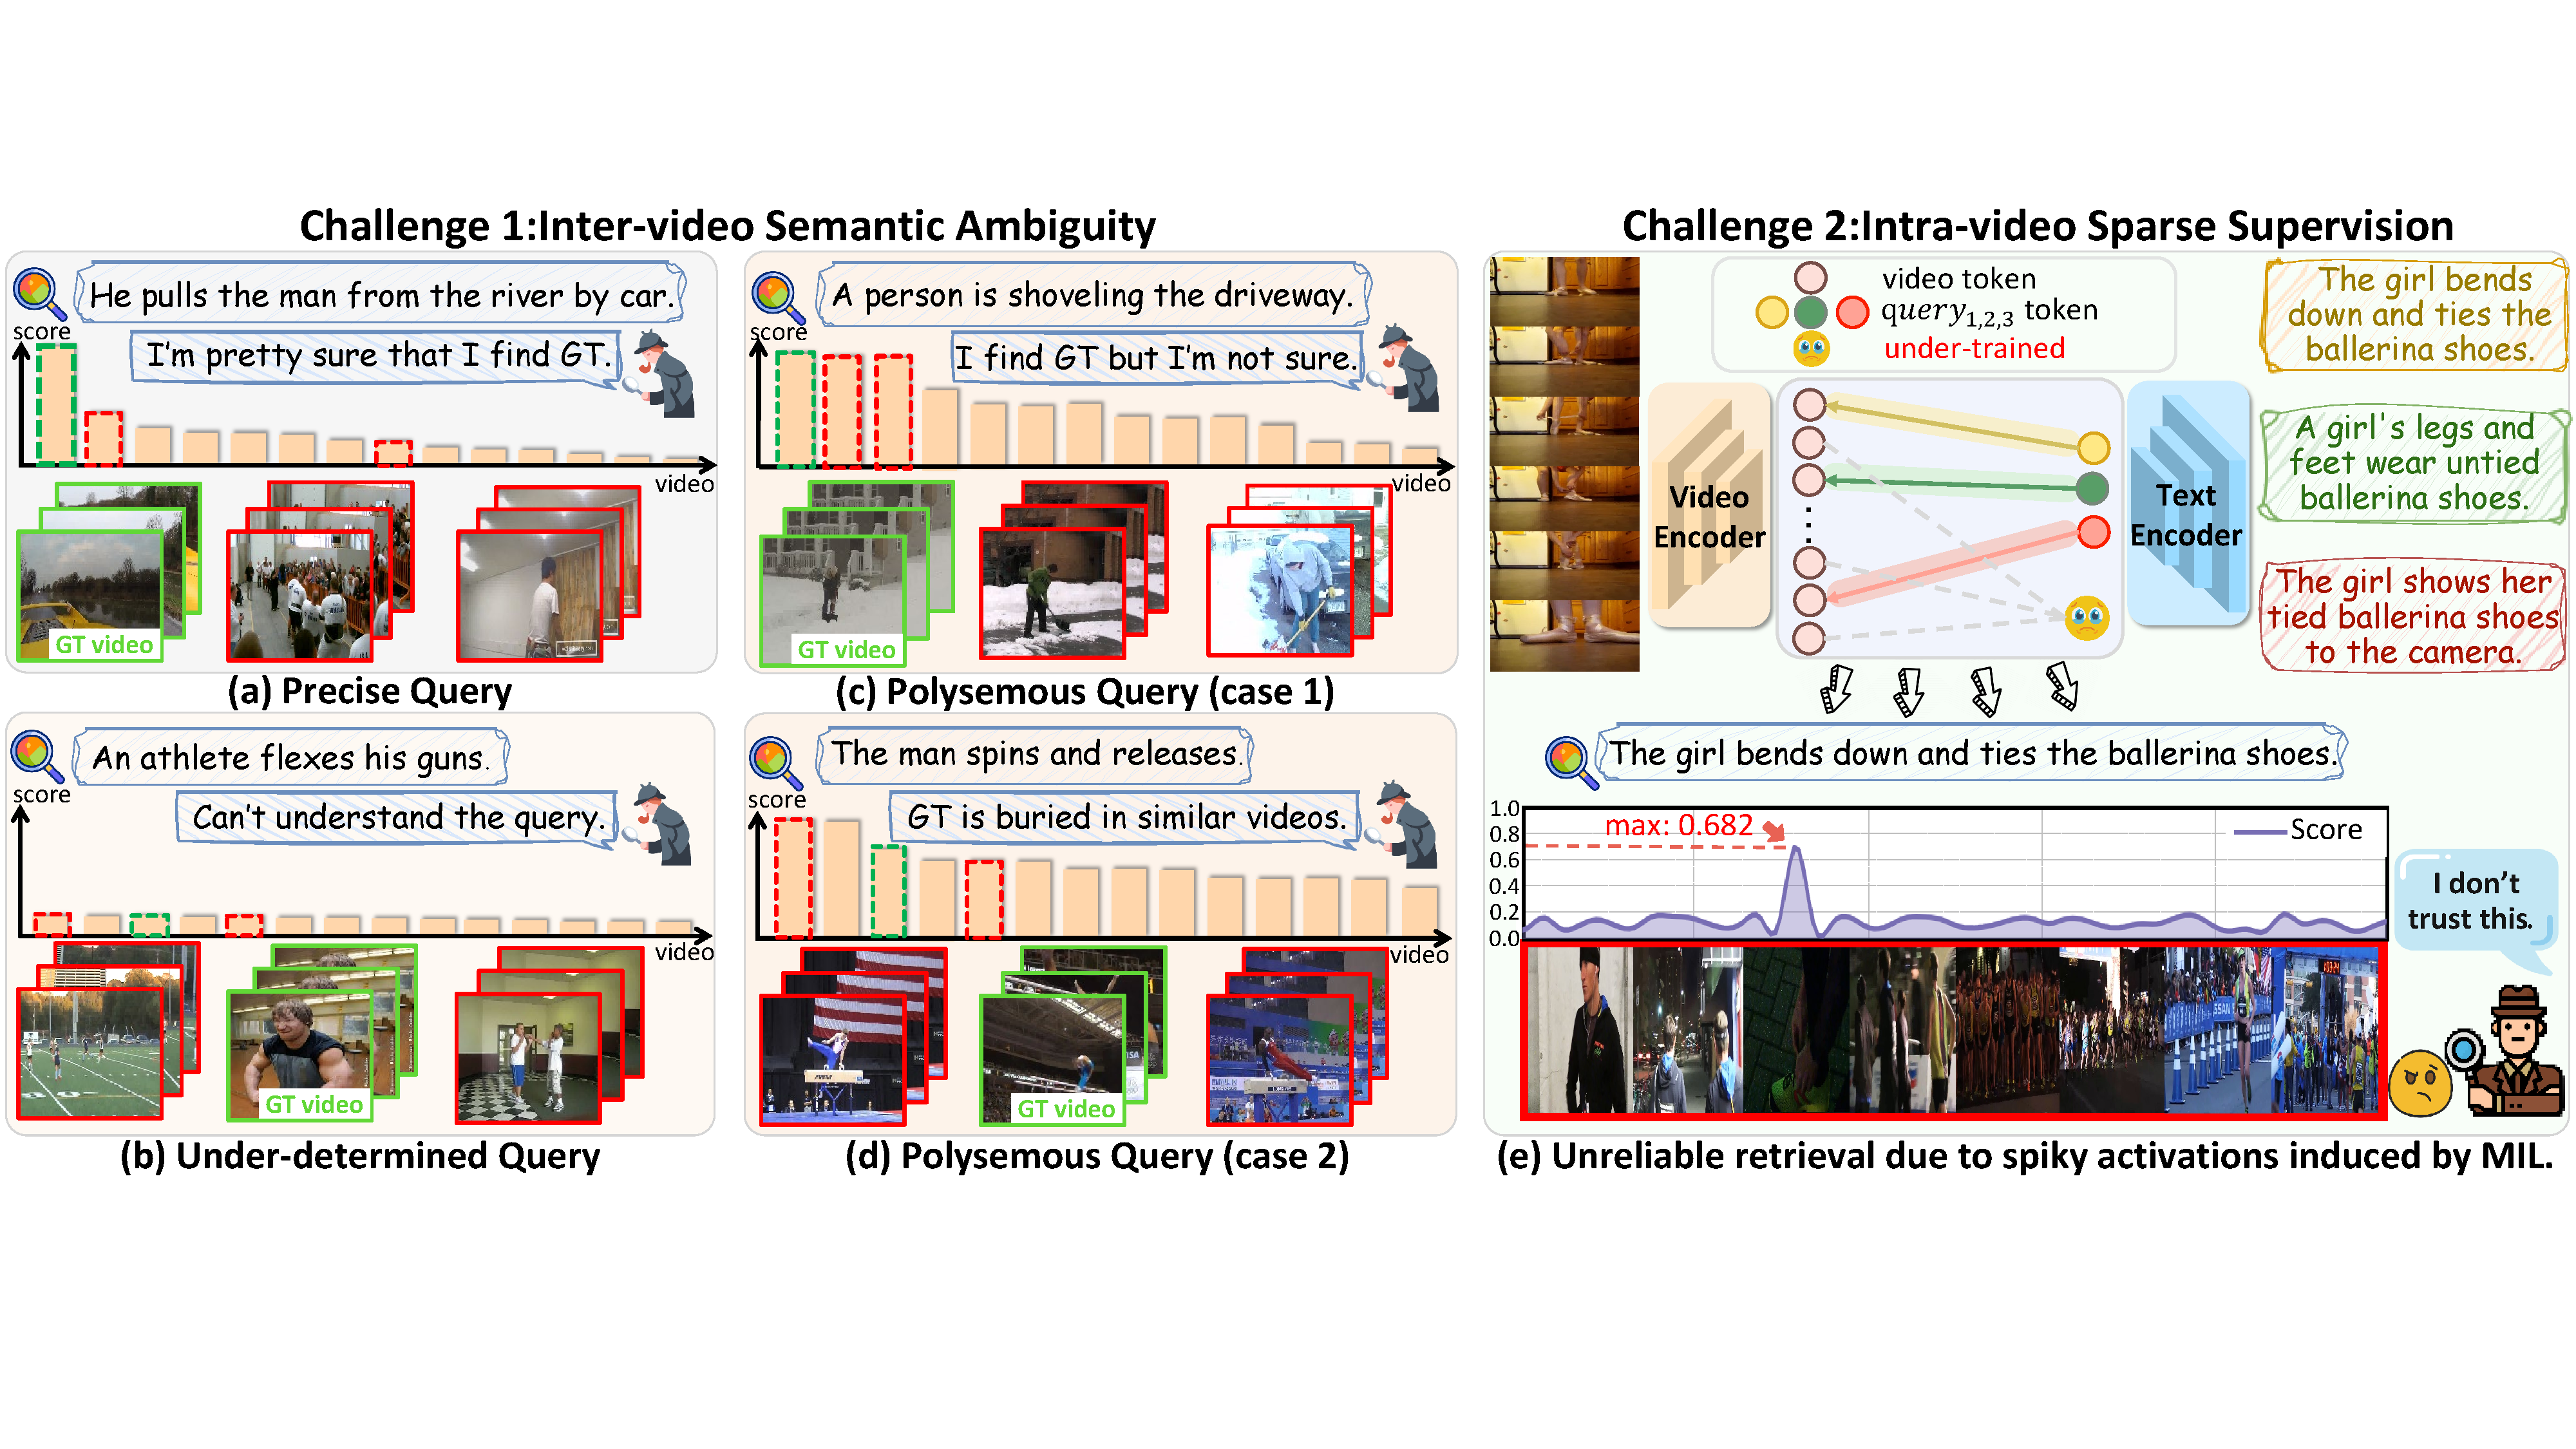
\includegraphics[width=\textwidth]{images/introv3.pdf}
    \caption{(a) \emph{精确查询}产生明显的响应间隔，真实匹配视频的得分显著高于其余候选。
    (b) \emph{信息不足查询}难以被模型正确理解，导致相似度响应较弱，缺乏区分度。
    (c-d) \emph{多义查询}存在语义歧义，对应多个合理候选，需要\emph{进一步甄别}以处理相关不确定性。
    (e) MIL 只优化最相近的配对，造成\emph{监督稀疏}、片段训练不足。模型因而容易受到整体无关的“跑步”视频中的局部噪声干扰，产生虚假尖峰激活，降低检索可靠性。
    }
    \label{fig:Intro}
\end{figure*}

随着在线视频快速增长，文本到视频检索（T2VR）\cite{PIG}受到越来越多关注。大多数 T2VR 方法针对预先裁剪的视频和能够完整描述视频的查询而设计，难以直接对应现实场景。现实中的视频通常未经裁剪，查询也往往只对应其中某些片段。因此，研究者提出了\emph{部分相关视频检索}（PRVR）\cite{ms-sl}，旨在根据描述部分内容的查询检索未经裁剪的视频。
这项任务的根本难点在于数据不对称。与内容丰富的视频相比，文本查询往往简短而含糊，检索过程因此具有内在的不确定性。

对此类不确定性建模需要同时解决视频间与视频内两个层面相互叠加的困难：
(\textbf{i}) \textbf{视频间语义歧义。} 由于内在的不确定性，查询之间常存在细粒度差异。\cref{fig:Intro}(a-d) 表明，除理想的\emph{精确查询}外，真实数据还包含\emph{信息不足查询}（语义信息不足、置信度低）和\emph{多义查询}（语义具有歧义、可以匹配多个候选）。多数既有方法忽略了这种差异\cite{GMMFORMER}，或借助正则化进行隐式处理\cite{RAL,msc-prvr}。ARL\cite{ARL}尝试识别存在歧义的视频与文本配对，但缺少显式量化具体不确定性类型的机制。
(\textbf{ii}) \textbf{视频内监督稀疏。} 视频内部缺少可靠证据，也会加剧视频间歧义。常用的多实例学习（MIL）范式只监督最匹配的单个片段，导致\emph{监督稀疏}。如\cref{fig:Intro}(e) 所示，监督失衡限制了训练信号，使模型难以学习整体表征，容易被虚假的局部噪声干扰。虽然从 CLIP\cite{CLIP} 蒸馏线索可以缓解稀疏性\cite{DL-DKD}，但帧级线索过于零散，无法捕捉确认视频相关性所需的时序变化，进而加剧视频间不确定性，影响检索表现。


为解决上述问题，我们认为模型需要在确定性的相似度分数之外，进一步评估预测的不确定性。本文提出统一的证据学习框架 \modelname{}，在两个层面区分并建模不确定性。
首先，为处理\textbf{视频间不确定性}，我们将跨模态相似度视为证据，并用 Dirichlet 分布进行参数化。由此，模型可以在计算匹配分数的基础上\emph{诊断}查询类型。我们提出不确定性引导识别（UGI）策略，依据\emph{认知不确定性}、\emph{标签一致性}与\emph{偶然不确定性}三项原则对查询分类，并进行查询自适应的标签校准。
其次，为缓解会加剧不确定性的\textbf{视频内监督稀疏}问题，我们试图积累更密集的证据。我们制定灵活最优传输（FOT）方案，在查询与多个相关片段之间建立软对齐。为提高抗噪能力，我们引入\emph{回收槽}吸收无关片段，从而提供更加全面、可靠的时序监督。

我们在 ActivityNet Captions\cite{krishna2017dense}、Charades-STA\cite{gao2017tall} 和 TVR\cite{lei2020tvr} 上开展了大量实验，结果表明 \modelname{} 达到当前先进水平。在标准检索指标之外，进一步分析表明，\modelname{} 能够有效解释查询歧义，并抑制 MIL 中的虚假激活。

本文的主要贡献如下：
\vspace{-.2cm}
\begin{itemize}
    \item[$\bullet$] \emph{\textbf{概念层面}}：我们从不确定性的角度重新审视 PRVR，明确联系了视频间语义歧义和视频内监督稀疏。 \vspace{-.2cm}
    \item[$\bullet$] \emph{\textbf{方法层面}}：我们提出双层证据学习框架 \modelname{}，通过三项判别原则实现细粒度的查询识别和标签校准，再用灵活最优传输构建密集、稳健的时序对齐。\vspace{-.2cm}
    \item[$\bullet$] \emph{\textbf{实验层面}}：\modelname{} 在三个基准上均取得了显著提升。细致的消融研究还验证了它量化查询不确定性以及抑制虚假局部噪声的能力。
\end{itemize}
\section{相关工作}
\label{sec:related_works}
\noindent \textbf{部分相关视频检索} \quad
传统的文本到视频检索（T2VR）方法\cite{Video-ColBERT,PIG,BLiM}检索与查询完全相关、预先裁剪的视频。由 MS-SL\cite{ms-sl} 首次提出的部分相关视频检索（PRVR）\cite{dreamprvr,sdm-prvr,bgmnet,amdnet,PEAN}则面向未经裁剪的视频，其中只有部分片段与查询匹配。视频语料库时刻检索（VCMR）\cite{zhang2025video,jsg}是另一项受到广泛研究的检索任务，旨在从大型视频语料库中定位特定时刻。PRVR 与 VCMR 的第一阶段类似，二者均进行粗粒度的视频级检索。但 VCMR 需要时刻级标注，因此更难扩展。

既有 PRVR 方法主要关注片段建模，很少考虑语义歧义。MS-SL\cite{ms-sl,MS-SL++} 通过滑动窗口构建带有冗余的片段嵌入，而 ProtoPRVR\cite{ProtoPRVR} 通过生成少量原型加速检索。GMMFormer\cite{GMMFORMER,GMMFormerV2} 使用高斯注意力隐式建模片段。
RAL\cite{RAL} 利用概率嵌入，MSC-PRVR\cite{msc-prvr} 则通过辅助训练损失缓解语义坍缩，两者均对查询歧义进行隐式建模；ARL\cite{ARL} 显式识别有歧义的查询与视频配对。然而，这些方法未能细分查询类别，也忽视了多实例学习导致的监督稀疏，限制了检索性能。我们提出 \modelname{}，以视频间证据学习识别查询差异，并以视频内证据学习构建查询与片段之间的软关联，提供更密集的监督信号。

\noindent \textbf{不确定性学习} \quad
尽管深度神经网络应用广泛，其预测大多是确定性的，缺少显式量化不确定性的机制。早期研究主要依赖贝叶斯神经网络（BNN）\cite{BNN} 和蒙特卡洛 Dropout\cite{montedropout2}。近年来，证据深度学习（EDL）\cite{edl-2018}受到越来越多关注。它以 Dempster-Shafer 理论（DST）\cite{dst} 和主观逻辑（SL）\cite{sl} 为基础，利用二阶概率分布显式建模不确定性，并已成功应用于多视图分类\cite{tmc,rcml}、噪声对应下的多模态检索\cite{rule,tcl,decl,ugncl,ucpm}、时序动作定位\cite{chenlo1,chenlo2}、开放集动作识别\cite{osa1,osa2}和零样本学习\cite{crest}等任务。后续研究\cite{fisher-edl,r-edl,flex-edl}进一步提高了 EDL 估计不确定性的能力。
受这些进展启发，我们设计了分层证据学习框架，汇聚不同粒度的跨模态证据，共同量化 PRVR 中的检索不确定性。

\section{方法}
\subsection{问题定义与框架概览} \label{subsec:overview}
\begin{figure*}[t]
    \centering
    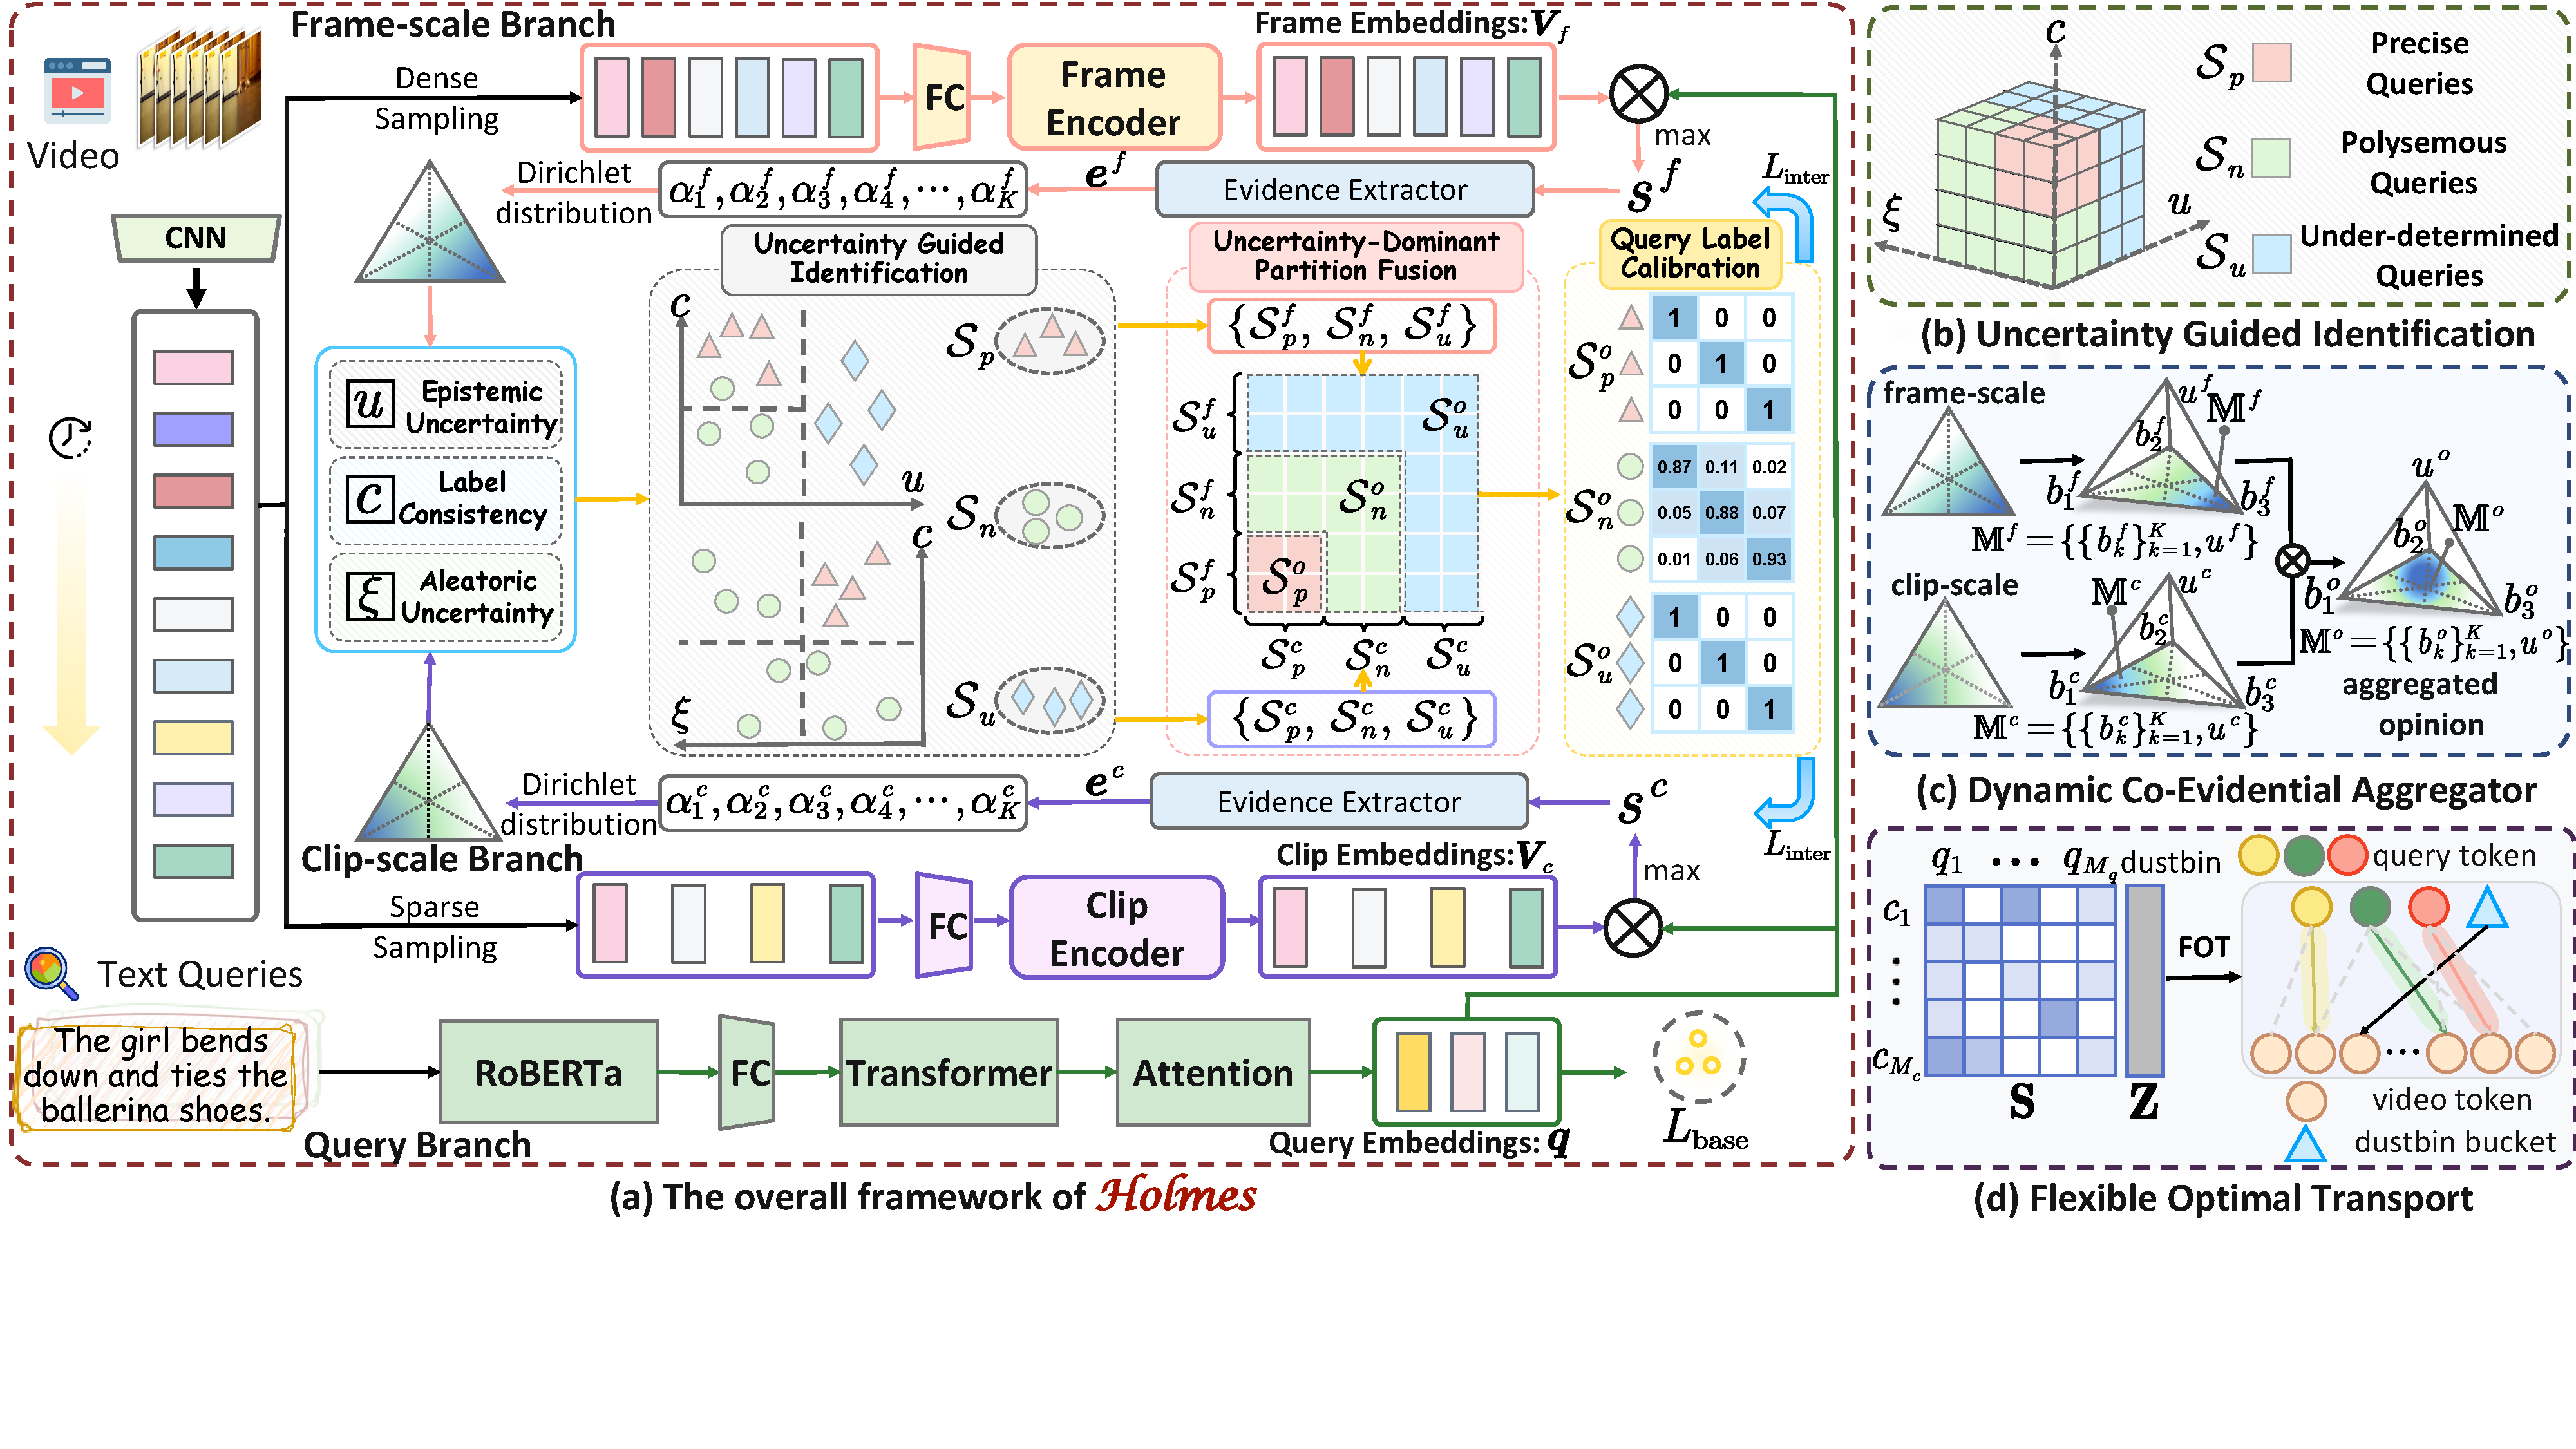
\includegraphics[width=\textwidth]{images/methodv3.pdf}
    \caption{\modelname{} 框架概览。
\textbf{(a)} 查询分支生成查询嵌入 $\bmq$，帧与片段尺度分支分别提取视频表征 $\bmV_f$ 和 $\bmV_c$，得到相似度分数 $S_f$ 和 $S_c$。将候选相似度转换为证据向量，以 Dirichlet 分布建模并估计三项判别量。不确定性引导识别据此将各尺度查询划分为精确查询（$\mathcal{S}^f_p$、$\mathcal{S}^c_p$）、多义查询（$\mathcal{S}^f_n$、$\mathcal{S}^c_n$）和信息不足查询（$\mathcal{S}^f_u$、$\mathcal{S}^c_u$）。不确定性主导的划分融合整合两种尺度的划分，得到 $\mathcal{S}^o_p$、$\mathcal{S}^o_n$ 和 $\mathcal{S}^o_u$。完成查询自适应的标签校准后，以修正后的标签通过 $L_{\mathrm{inter}}$ 监督视频间证据学习。
\textbf{(b)} 不确定性引导识别在三维潜在空间中划分查询，先在 $c$--$u$ 平面上粗分，再沿 $\xi$ 轴细分。
\textbf{(c)} 动态协同证据聚合器无需额外参数，即可融合两种尺度的证据意见。
\textbf{(d)} 灵活最优传输使用\emph{回收槽}吸收噪声片段，将可靠的查询与片段软分配作为视频内证据学习的标签证据。
    }
    \label{fig:arc}
\end{figure*}
部分相关视频检索旨在找出包含给定文本查询所描述时刻的视频。每个视频包含多个候选时刻，而每条查询对应相关视频中的某个特定时刻。本文提出分层证据学习框架 \modelname{}，从视频间和视频内两个层面处理 PRVR 的查询歧义，如\cref{fig:Intro}(a) 所示。下面先介绍三个组成部分。

\noindent \textbf{文本查询表征} \quad
先使用预训练的 RoBERTa~\cite{liu2019roberta} 对文本查询编码，再通过投影层和 Transformer~\cite{vaswani2017attention} 获取上下文化表征。与 MS-SL\cite{ms-sl} 类似，最终将表征聚合成 $\bmq \in \mathbb{R}^d$。

\noindent \textbf{视频表征} \quad 对于未经裁剪的视频，先用预训练 CNN 提取特征。参照已有工作\cite{GMMFORMER}，我们采用双分支架构提取多尺度表征。
帧尺度分支通过全连接层将采样所得的 $M_f$ 帧投影到 $d$ 维空间，再由帧编码器得到 $\bm{V_f} = \{\bmf_i\}_{i=1}^{M_f} \in \mathbb{R}^{M_f \times d}$。
片段尺度分支将视频稀疏划分成 $M_c$ 个片段，投影后送入片段编码器，得到 $\bm{V_c} = \{\bmc_i\}_{i=1}^{M_c} \in \mathbb{R}^{M_c \times d}$。

\noindent \textbf{相似度计算} \quad
为计算文本与视频配对 $(T, V)$ 的相似度，先获得 $\bmq$、$\bm{V_f}$ 和 $\bm{V_c}$，再计算帧尺度与片段尺度的相似度分数：
\vspace{-.6em}
\begin{equation}
\begin{aligned}
s^f(T, V) = \text{max} \{ \text{cos}(\bmq, \bmf_1),..., \text{cos}(\bmq, \bmf_{M_f})\}, \\
s^c(T, V) = \text{max} \{\text{cos}(\bmq, \bmc_1),..., \text{cos}(\bmq, \bmc_{M_c})\}.
\label{eq:simscore}
\end{aligned}
\vspace{-.6em}
\end{equation}
随后计算文本与视频之间的总体相似度分数：
\vspace{-.6em}
\begin{equation}\label{eq:sim}
s({T}, {V}) = \alpha_f s^f({T}, {V}) + \alpha_c s^c({T}, {V}),
\vspace{-.6em}
\end{equation}
其中 $\alpha_f, \alpha_c \in [0,1]$，且 $\alpha_f + \alpha_c = 1$。最终按\cref{eq:sim} 给出的分数检索并排序视频。

\subsection{视频间证据学习}
本节通过视频间证据学习估计查询的不确定性，以此对查询歧义建模。我们先介绍查询识别的三项判别原则（\cref{fig:arc}(a)）。两个分支流程相似，以下以帧尺度分支为例。

\noindent \textbf{三项判别原则} \quad
对于查询 $\bmq_i$ 和 $K$ 个视频，先计算查询与第 $j$ 个视频的帧尺度相似度 $s^f_{ij}$（\cref{eq:simscore}），简记为 $s_{ij}$。
% Viewing retrieval as $K$-class classification,
沿用\citep{edl-2018} 的做法，从相似度导出证据：
\vspace{-.8em}
\begin{equation}
    e_{ij} = \exp\left(\tanh\left(s_{ij}/ \tau\right)\right), \quad 
    \boldsymbol{e}_i = [e_{i1}, \dots, e_{iK}],
    \vspace{-.8em}
    \label{ea:evi1}
\end{equation}
默认设 $\tau=0.1$。根据 Dempster-Shafer 理论（DST）\cite{dst}，可利用证据量化认知不确定性，反映数据对查询与候选视频关联的支持程度。
% Following Subjective Logic (SL) \cite{ edl-2018}, 
首先将证据 $ {e}_i$ 映射为 Dirichlet 分布参数：
\vspace{-.8em}
\begin{equation}
    {\boldsymbol \alpha}_i = [\alpha_{i1}, \dots, \alpha_{iK}], \quad \alpha_{ij} = e_{ij}+1.
    \label{eq:dir-alpha}
    \vspace{-.6em}
\end{equation}
\begin{definition}\textbf{认知不确定性。} 对于查询 $\bmq_i$，认知不确定性 $u_i$ 和信念质量 $b_{ij}$ 定义为
\vspace{-1.em}
\begin{equation}
    u_i = \frac{K}{S_i}, \quad b_{ij} = \frac{\alpha_{ij}-1}{S_i}, \quad 
    S_i = \sum_{j=1}^{K} \alpha_{ij},
    \label{eq:dir-alpha2}
\vspace{-1.em}
\end{equation}
且 $u_i + \sum_{j} b_{ij} = 1$。这里，$S_i$ 表示 Dirichlet 分布的强度，$ {\boldsymbol b}_i = [b_{i1}, \dots, b_{iK}]$ 表示由 $ {\boldsymbol \alpha}_i$ 导出的主观意见。
\vspace{-.8em}
\end{definition}
较高的 $u_i$ 反映证据有限、模型对查询理解不足，可用于识别信息不足查询。但 $u_i$ 较低并不能保证检索精确。形式化地说：
\vspace{-.6em}
\begin{theorem}
较低的认知不确定性 $u_i$ 并不意味着最高信念一定分配给标注标签 $ {y}_{i}$。
\vspace{-.8em}
\begin{equation}
    \boldsymbol q_i \text{ 的 } u_i \text{ 较低} \nRightarrow \arg\max\, \boldsymbol{b}_{i} = \arg\max \boldsymbol{y}_{i}.
\vspace{-.8em}
\end{equation}
\label{theorem: wrong uncertainty}
\end{theorem}
\vspace{-2em}
证明见附录 \ref{appendix:theorem3.2}。$\boldsymbol{y}_i = [y_{i1}, \dots, y_{iK}]$ 是独热真实标签。该定理表明，仅凭认知不确定性无法保证信念集中在标注视频上，因此我们引入标签一致性原则。
\begin{definition} \textbf{标签一致性。} 对于查询 $\bmq_i$，标签一致性 $c_i$ 定义为：
\vspace{-.6em}
    \begin{equation}
        c_{i}=\max (0, \boldsymbol{s}_{i}\cdot \boldsymbol{y}_{i}),
        \label{eq: cons}
\vspace{-.6em}
    \end{equation}
其中 $\boldsymbol{s}_i = [s_{i1}, \dots, s_{iK}]$ 表示相似度分数。
\vspace{-.6em}
\end{definition}
较低的 $c_i$ 表明查询与真实匹配视频的对齐较差，但较高的 $c_i$ 并不能说明查询精确。形式化地说：
\begin{proposition}
较高的标签一致性 $c_i$ 并不意味着该查询是精确查询。
\vspace{-.6em}
\begin{equation}
    \boldsymbol q_i \text{ 的 } c_i \text{ 较高} \nRightarrow \boldsymbol q_i \text{ 是精确查询}.
    \vspace{-.8em}
\end{equation}
\label{theorem:wrong-consistency}
\vspace{-2em}
\end{proposition}
\vspace{-.6em}
\begin{proof} 如\cref{fig:Intro}(c) 所示，真实匹配视频的响应较高并不意味着匹配精确，因为其他视频也可能具有同样高的相似度。
\vspace{-1em}
\end{proof}
为区分精确查询和多义查询，我们引入偶然不确定性\cite{au}，用\cref{eq:aleatoric-uncertainty} 中 $\text{Dir}({\boldsymbol\alpha_i})$ 下的期望熵来衡量。低熵表示概率质量集中于单个视频，表明查询可能是精确的。高熵则表示概率分布较为均匀，表明查询可能存在多义性。

\begin{definition} \textbf{偶然不确定性。}
对于查询 $\bmq_i$，偶然不确定性 $\xi_i$ 定义为
\vspace{-.6em}
\begin{equation}
\!\!\!\!\mathbb{E}_{\mathbf{p} \sim \text{Dir}({\boldsymbol\alpha_i})} [H(\mathbf{p})]\!\!=\!\!\sum_{k=1}^K \frac{\alpha_{ik}}{S_{i}} \left( \psi(S_{i} \!+ \!1) \!-\! \psi(\alpha_{ik}\! + \!1) \right),
\vspace{-.6em}
\label{eq:aleatoric-uncertainty}
\end{equation}
其中 $\psi$ 表示 digamma 函数，定义为 $\psi(x) = \frac{d}{d x} \log \Gamma(x)$，$H$ 表示 Shannon 熵。完整推导见附录 \ref{appendix:aleatoric-uncertainty}。
\vspace{-.6em}
\end{definition}

\noindent \textbf{不确定性引导识别} \quad \label{method:ugi}
依据上述原则，可将查询分为三类：
(i) 认知不确定性较高的信息不足查询 $\mathcal{S}_{u}$；
(ii) 认知不确定性较低、标签一致性较高的初步精确查询 $\mathcal{\tilde{S}}_{p}$；
(iii) 认知不确定性较低、标签一致性较低的初步多义查询 $\mathcal{\tilde{S}}_{n}$。
形式化表示如下：
\vspace{-.6em}
\begin{equation}
\begin{cases} 
\mathcal{S}_{u} = \{q_i \mid u_i > \beta_u\}, \\ 
\mathcal{\tilde{S}}_{p} = \{q_i \mid u_i \le \beta_u,\, c_i \ge \beta_p\}, \\
\mathcal{\tilde{S}}_{n} = \{q_i \mid u_i \le \beta_u,\, c_i < \beta_p\}.
\end{cases}    
\label{eq:initial-division}
\vspace{-.6em}
\end{equation}
阈值 $\beta_u$ 和 $\beta_p$ 按以下方式自适应确定：
\vspace{-.6em}
\begin{equation}
    \beta_u = \min(u^{tp}, 1 - \beta), \quad 
    \beta_p = \max(\beta, c^{tp}),
    \label{eq:threshold}
\vspace{-.6em}
\end{equation}
其中 $u^{tp}$=$\max_{i \in \mathcal{S}^{tp}} u_i$，$c^{tp}$ = $\min_{i \in \mathcal{S}^{tp}} c_i$，且 $\beta=0.3$。$\mathcal{S}^{tp}= \left\{ i \,\middle|\, \arg\max(\boldsymbol{s}_i) = \arg\max(\boldsymbol{y}_i) \right\}$ 表示正确匹配的查询与视频配对。在噪声对应学习中，$\mathcal{\tilde{S}}_{n}$ 通常被视为噪声配对，我们则将其解释为查询歧义的表现。含糊的语义可能削弱真实匹配视频的响应。命题 \ref{theorem:wrong-consistency} 表明，$\mathcal{\tilde{S}}_{p}$ 中也仍包含多义查询。进一步比较 $\xi$，对 $\mathcal{\tilde{S}}_{p}$ 细分，得到最终的精确查询集合 $\mathcal{S}_{p}$ 和多义查询集合 $\mathcal{S}_{n}$：
\vspace{-.6em}
\begin{equation}
\begin{cases}
\mathcal{S}_p = \{ q_i \in \mathcal{\tilde{S}}_p \mid \xi_i < \text{median}(\{\xi_j\}_{q_j \in \mathcal{\tilde{S}}_p}) \}, \\
\mathcal{S}_n = \bigl( \mathcal{\tilde{S}}_p \cup \mathcal{\tilde{S}}_n \bigr) \setminus \mathcal{S}_p.
\end{cases}
\label{eq:refined_partition}
\vspace{-.6em}
\end{equation}
\noindent\textbf{不确定性主导的划分融合} \quad
根据\cref{eq:initial-division,eq:refined_partition}，帧尺度与片段尺度分支分别生成查询划分 $\{\mathcal{S}_u^f, \mathcal{S}_p^f, \mathcal{S}_n^f\}$ 和 $\{\mathcal{S}_u^c, \mathcal{S}_p^c, \mathcal{S}_n^c\}$。
对于同一查询，两个分支可能给出不一致的预测，因此需要一套原则来协调分歧。

% \vspace{-.6em}
\begin{definition}\textbf{不确定性主导次序。}
\label{def:uncertainty_order}
在查询类别上定义\emph{不确定性主导次序}：
\vspace{-.6em}
\begin{equation}
    \mathcal{S}_p \;\prec\; \mathcal{S}_n \;\prec\; \mathcal{S}_u ,
    \vspace{-.6em}
\end{equation}
该次序按语义歧义与不确定性递增构成全序。
\vspace{-.5em}
\end{definition}
这样的排序源自以下观察：精确查询的语义可靠，多义查询对应多个合理候选，信息不足查询则缺少足以支持高置信匹配的证据。因此，当两个分支的判别结果冲突时，选择不确定性更高的类别：
% Accordingly, when the two branches produce conflicting predictions, we resolve the disagreement by selecting the identification with the higher uncertainty dominance:
\vspace{-.6em}
\begin{equation}
\begin{cases}
\mathcal{S}^o_p = \mathcal{S}_p^f \cap \mathcal{S}_p^c, \\
\mathcal{S}^o_n = (\mathcal{S}_n^f \cap \mathcal{S}_p^c)
               \;\cup\; (\mathcal{S}_p^f \cap \mathcal{S}_n^c)
               \;\cup\; (\mathcal{S}_n^f \cap \mathcal{S}_n^c), \\
\mathcal{S}^o_u= \begin{aligned}[t]
  & \bigl(\mathcal{S}_u^f \cap \mathcal{S}_u^c\bigr) \cup \bigl(\mathcal{S}_u^f \cap (\mathcal{S}_p^c \cup \mathcal{S}_n^c)\bigr) \\
  & \cup \bigl( \mathcal{S}_u^c \cap (\mathcal{S}_p^f \cup \mathcal{S}_n^f)\bigr). \\
\end{aligned}
\end{cases}
\label{eq:influence_fusion}
\vspace{-.6em}
\end{equation}
\noindent \textbf{查询标签校准} \quad
得到最终的 $\mathcal{S}^o_p$、$\mathcal{S}^o_n$ 和 $\mathcal{S}^o_u$ 后，我们按查询类型进行标签校准。对 $\mathcal{S}^o_p$ 中的精确查询，保留原始标签。$\mathcal{S}^o_u$ 中的信息不足查询因语义证据匮乏而仍处于欠拟合状态，也保留其原始标签以促进学习。
对于 $\mathcal{S}^o_n$ 中的多义查询，独热监督忽视语义歧义，可能过度惩罚语义相关的样本，并引入误导性监督。我们利用模型估计的相似度重新校准这些标签，产生能够反映潜在相关性的软对齐概率。
给定标签为 $y_i$ 的第 $i$ 条查询，修正后的标签 $\hat{\boldsymbol{y}}_i$ 为：
\vspace{-.5em}
\begin{equation}
   \!\!\! \hat{\boldsymbol{y}}_i \!\!=\!\!
    \begin{cases}
        \boldsymbol{y}_i, \!\!& \!\!i \in \mathcal{S}^o_p \cup \mathcal{S}^o_u, \\
        \!(\!1-\gamma\!) \boldsymbol{y}_i
        + \dfrac{\gamma}{2}\!\left(\sigma(s^f_i) + \sigma(s^c_i)\right), \!\!
        & \!\!i \in \mathcal{S}^o_n ,
    \end{cases}
    \label{eq:ref_label}
\vspace{-.5em}
\end{equation}
其中 $\sigma(\cdot)$ 表示 softmax 运算，$\gamma$ = 0.2。$s^f_i$ 和 $s^c_i$ 分别为帧尺度与片段尺度的相似度分数。

\noindent \textbf{动态协同证据聚合器} \quad 如\cref{fig:arc}(c) 所示，给定查询 $\bmq$，先根据\cref{eq:dir-alpha,eq:dir-alpha2} 获得帧尺度和片段尺度的证据意见 $\mathbb{M}^f = \big\{\{b_k^f\}_{k=1}^{K}, u^f\big\}$ 和 $\mathbb{M}^c = \big\{\{b_k^c\}_{k=1}^{K}, u^c\big\}$。
然后按 Dempster-Shafer 理论的组合规则融合两个分支的意见，得到 $\mathbb{M}^o = \big\{\{b_k^o\}_{k=1}^{K}, u^o\big\}$：
\vspace{-.5em}
\begin{equation}
b^o_{k}=\frac{1}{1-\delta}( b^f_kb^c_k + b^f_ku^c + b^c_ku^f), u^o = \frac{1}{1-\delta}u^fu^c,
\vspace{-.5em}
\end{equation}
其中 $\delta = \sum_{i\neq j}{b^f_i b^c_j}$ 衡量两种意见的冲突程度。融合意见可反映查询的整体不确定性，并作为全局监督信号协调两个分支。

获得多尺度证据意见，完成查询分类和标签校准后，我们定义证据学习目标。将跨模态检索表述为 $K$ 类分类问题，通过最小化基于 Dirichlet 分布的查询概率 $\boldsymbol{p}_i$ 与校准标签 $\hat{\boldsymbol{y}}_i$ 之间的最小二乘损失来优化 \modelname{}：
\vspace{-.6em}
\begin{equation}
   \!\!\! \begin{aligned}
        {L}_{U}(\boldsymbol{\alpha}_{i},{\hat{\boldsymbol y}}_{i})&=\int\left\|\hat{\boldsymbol y}_i-\boldsymbol{p}_i\right\|_2^2 \frac{1}{B\left(\boldsymbol{\alpha}_i\right)} \prod_{j=1}^{K} p_{i j}^{\alpha_{i j}-1} d \boldsymbol{p}_i \\
        & = \sum_{j=1}^{K} \left(\hat{y}_{i j}-\frac{\alpha_{i j}}{S_i}\right)^2+\frac{\alpha_{i j}\left(S_i-\alpha_{i j}\right)}{S_i^2\left(S_i+1\right)}.
    \end{aligned}
    \label{eq:evi-loss}
\vspace{-.6em}
\end{equation}
更多细节见附录 \ref{appendix:equation17}。\cref{eq:evi-loss} 约束匹配配对的证据高于不匹配配对，从而维持不确定性学习的可靠性。最后，第 $i$ 条查询的视频间证据学习总体目标为：
\vspace{-.6em}
\begin{equation}
    {L}_{\mathrm{inter}} =
    {L}^f_{U}\!\left(\boldsymbol{\alpha}^{f}_{i}, \hat{\boldsymbol{y}}_{i}\right)
    + {L}^c_{U}\!\left(\boldsymbol{\alpha}^{c}_{i}, \hat{\boldsymbol{y}}_{i}\right)
    + {L}^o_{U}\!\left(\boldsymbol{\alpha}^{o}_{i}, \hat{\boldsymbol{y}}_{i}\right),
\vspace{-.6em}
\end{equation}
其中 $\boldsymbol{\alpha}^{f}_{i}$、$\boldsymbol{\alpha}^{c}_{i}$ 和 $\boldsymbol{\alpha}^{o}_{i}$ 分别是帧尺度、片段尺度和融合证据意见对应的 Dirichlet 参数。


\begin{table*}[t]
\caption{\textbf{三个标准数据集上的检索性能对比。} 模型按 ActivityNet Captions 上的 SumR 升序排列。粗体表示最佳结果，短横线表示未提供结果。}
\label{tab:main}
\centering
\resizebox{\textwidth}{!}{
\begin{tabular}{l ccccc c ccccc c  ccccc}
\toprule
\multirow{2}{*}{\textbf{模型}}& \multicolumn{5}{c}{\textbf{ActivityNet Captions}} &  & \multicolumn{5}{c}{\textbf{Charades-STA}}&& \multicolumn{5}{c}{\textbf{TVR}} \\
\cmidrule{2-6} \cmidrule{8-12} \cmidrule{14-18}
& \textbf{R@1} & \textbf{R@5} & \textbf{R@10} & \textbf{R@100} & \textbf{SumR} && \textbf{R@1} & \textbf{R@5} & \textbf{R@10} & \textbf{R@100} & \textbf{SumR} & & \textbf{R@1} & \textbf{R@5} & \textbf{R@10} & \textbf{R@100} & \textbf{SumR} \\
\midrule
\midrule

\rowcolor{basegray}
\multicolumn{18}{l}{\scalebox{1.15}{\textit{文本到视频检索（T2VR）}}}\\
RIVRL \cite{dong2022reading} & 5.2 & 18.0 & 28.2 & 66.4 & 117.8 &&1.6 & 5.6 & 9.4 & 37.7  & 54.3 && 9.4 & 23.4 & 32.2 & 70.6 & 135.6  \\
CLIP4Clip \cite{luo2022clip4clip} & 5.9 & 19.3 & 30.4 & 71.6 & 127.3 &&1.8 & 6.5 & 10.9 & 44.2 & 63.4 &&  9.9 & 24.3 & 34.3 & 72.5 & 141.0\\
Cap4Video  \cite{wu2023cap4video} & 6.3 & 20.4 & 30.9 & 72.6 & 130.2 &&1.9 & 6.7 & 11.3 & 45.0 & 65.0 &&  10.3 & 26.4 & 36.8 & 74.0 & 147.5\\
\midrule

\rowcolor{basegray}
\multicolumn{18}{l}{\scalebox{1.15}{\textit{视频语料库时刻检索（VCMR）}}}\\
ReLoCLNet \cite{zhang2021video} & 5.7 & 18.9 & 30.0 & 72.0 & 126.6 &&1.2 & 5.4 & 10.0 & 45.6 & 62.3 & & 10.0 & 26.5 & 37.3 & 81.3  & 155.1 \\
CONQUER \cite{hou2021conquer}&  6.5 & 20.4 & 31.8 & 74.3  & 133.1 &&1.8 & 6.3 & 10.3 & 47.5  & 66.0 &&11.0 & 28.9 & 39.6 & 81.3  & 160.8 \\ 
JSG \cite{jsg}&  6.8 & 22.7 & 34.8 & 76.1  & 140.5 &&2.4 & 7.7 & 12.8 & 49.8  & 72.7 &&- & - & - & -  & -\\ 
\midrule

\rowcolor{basegray}
\multicolumn{18}{l}{\scalebox{1.15}{\textit{部分相关视频检索（PRVR）}}}\\
MS-SL \cite{ms-sl}& 7.1 & 22.5 & 34.7 & 75.8 & 140.1 &&1.8 & 7.1 & 11.8 & 47.7 & 68.4& & 13.5 & 32.1 & 43.4 & 83.4 & 172.4       \\
MS-SL++ \cite{MS-SL++}& 7.0 & 23.1 & 35.2 & 75.8 & 141.1 && 1.8 & 7.6 & 12.0 & 48.4 & 69.7 && 13.6 & 33.1 & 44.2 & 83.5 & 174.5\\
 PEAN \cite{PEAN}&7.4 & 23.0 & 35.5 & 75.9 & 141.8 &&  \textbf{2.7} & 8.1 & 13.5 & 50.3 & 74.7 && 13.5 & 32.8 & 44.1 & 83.9 & 174.2 \\
  LH \cite{lh}& 7.4 & 23.5 & 35.8 & 75.8 & 142.4 &&2.1 & 7.5 & 12.9 & 50.1 & 72.7& & 13.2 & 33.2 & 44.4 & 85.5 & 176.3 \\
 BGM-Net \cite{bgmnet}& 7.2 & 23.8 & 36.0 & 76.9 & 143.9 &&1.9 & 7.4 & 12.2 & 50.1 & 71.6 && 14.1 & 34.7 & 45.9 & 85.2 & 179.9 \\
 GMMFormer \cite{GMMFORMER}&8.3 & 24.9 & 36.7 & 76.1 & 146.0 && 2.1 & 7.8 & 12.5 & 50.6 & 72.9 &&13.9 & 33.3 & 44.5 & 84.9 & 176.6 \\
 MamFusion \cite{mamfusion} &8.0 & 25.4 & 37.2 & 76.8 & 147.4 && 2.0 & 8.8 & 14.2 & 51.5 & 76.5 &&14.2 & 33.9 & 44.9 & 84.5 & 177.5 \\
 ProtoPRVR \cite{ProtoPRVR} & 7.9 & 24.9 & 37.2 & 77.3 & 147.4 && - & - & - & - & - && 15.4 & 35.9 & 47.5 & 86.4 & 185.1\\
 DL-DKD \cite{DL-DKD}& 8.0 & 25.0 & 37.5 & 77.1 & 147.6 &&- & - & - & - & - && 14.4 & 34.9 & 45.8 & 84.9 & 179.9  \\
ARL \cite{ARL}& 8.3 & 24.6 & 37.4 & 78.0 & 148.3 && - & - & - & - & - && 15.6 & 36.3 & 47.7 & 86.3 & 185.9\\
MGAKD \cite{MGAKD}& 7.9 & 25.7 & 38.3 & 77.8 & 149.6 && - & - & - & - & - && 16.0 & 37.8 & 49.2 & 87.5 & 190.5\\
DL-DKD++ \cite{dl-dkd++} & 8.3 & 25.5 & 38.3 & 77.8 & 149.9 && 1.9 & 7.1 & 12.3 & 49.8 & 71.1 && 15.3 & 36.0 & 47.5 & 86.0 & 184.8\\
GMMFormerV2 \cite{GMMFormerV2}& 8.9 & 27.1 & 40.2 & 78.7 & 154.9 && 2.5 & 8.6 & 13.9 & 53.2 & 78.2 && 16.2 & 37.6 & 48.8 & 86.4 & 189.1\\
HLFormer \cite{HLFormer}& 8.7 & 27.1 & 40.1 & 79.0 & 154.9 && 2.6 & 8.5 & 13.7 & 54.0 & 78.7 && 15.7 & 37.1 & 48.5 & 86.4 & 187.7\\
DreamPRVR \cite{dreamprvr} & 8.7 & 27.5 & 40.3 & 79.5 & 156.1 && 2.6 & 8.7 &14.5 &\textbf{54.2} &80.0 && 17.4 & 39.0 & 50.4 & 86.2 & 193.1\\
\rowcolor{ourscolor}
 \textbf{{\large \modelname{}} （本文）}& \textbf{9.3} & \textbf{27.8} & \textbf{40.5} & \textbf{79.1} & \textbf{156.8} &&2.3 & \textbf{9.5} & \textbf{15.2} & 53.6 & \textbf{80.6} &&   \textbf{18.4} & \textbf{40.7} & \textbf{52.0} & \textbf{87.5} & \textbf{198.6}     \\
\hline
\bottomrule
\end{tabular}
}
\end{table*}

\subsection{视频内证据学习}
为缓解 MIL 固有的监督稀疏问题，我们采用最优传输在每个视频内部建立查询与片段之间的软对齐。给定片段嵌入 $\{c_i\} \in \mathbb{R}^{M_c \times d}$ 及对应的查询嵌入 $\{q_j\} \in \mathbb{R}^{M_q \times d}$，其中 $M_q$ 表示查询数。设 $\mathbf{S} \in \mathbb{R}^{M_c \times M_q}$ 为片段与查询的相似度矩阵，$\mathbf{Q}$ 为传输分配矩阵。最优传输的目标为：
\vspace{-.6em}
\begin{equation}
\vspace{-.6em}
  \begin{aligned}
 \!\!\!\!&\max _{\mathbf{Q} \in \mathcal{Q}} \quad
 \langle\mathbf{Q},~ \mathbf{S}\rangle +\varepsilon H(\mathbf{Q})\\
\!\!\!\!&\text{s.t.}  \quad\!\!\!\!
\mathcal{Q}\!\!=\!\!\left\{\mathbf{Q}\! \in \!\mathbb{R}_{+}^{M_c \times M_q}\mid \mathbf{Q} \mathbf{1}_{M_q}=\boldsymbol{\mu}, \mathbf{Q}^{\top} \mathbf{1}_{M_c}= \boldsymbol{\nu} \right\},
\vspace{-.6em}
\end{aligned}
\label{eq:ot}
\end{equation}
其中 $\mathbf{1}_{M_q}$ 为 $M_q$ 维全一向量，$\boldsymbol{\mu}\in \mathbb{R}^{M_c}$，$\boldsymbol{\nu}\in \mathbb{R}^{M_q}$。$H(\mathbf{Q})$ 是熵正则项，$\varepsilon$ 控制平滑程度。通过 Sinkhorn 算法\citep{sinkhorn} 得到最优解 $\mathbf{Q}^*$。

\noindent \textbf{灵活最优传输} \quad
标准最优传输要求源端与目标端之间完全分配。这不适用于 PRVR，因为查询仅对应部分片段，其余片段可能包含噪声或冗余。受\cite{superglue,Nortorn} 启发，我们引入自适应回收槽以滤除这类片段，如\cref{fig:arc}(d) 所示。回收槽是一列由常数 $z$ 构成的向量，$z$ 取 $\mathbf{S}$ 的第 30 百分位值，然后将该列拼接到相似度矩阵：
\vspace{-.5em}
\begin{equation}
\bar{\mathbf{S}} = 
\begin{bmatrix}
\mathbf{S}\mid \mathbf{Z}
\end{bmatrix}, \quad
\mathbf{Z} = z \, \mathbf{1}_{{M_c} \times 1}.
\label{eq:new-s}
\vspace{-.5em}
\end{equation}
将\cref{eq:new-s} 的扩展矩阵用于\cref{eq:ot} 后，从解中去除回收槽，得到最终分配 $ {\bar{\mathbf{Q}}}^*= \bar{\mathbf{Q}}^*_{1: M_{c},1:{M_q}}$，从而实现一对多的软匹配。

将每次视频内对齐视为 $M_c$ 类分类，可按\cref{ea:evi1,eq:dir-alpha} 收集证据并估计 Dirichlet 参数。把 $ {{\bar{\mathbf{Q}}}^*}$ 作为校准后的标签，再根据\cref{eq:evi-loss} 定义视频内证据学习目标 $L_{\mathrm{intra}}$。对于每条查询，$L_{\mathrm{intra}}$ 鼓励模型为\emph{多个相关}片段积累强证据，为无关片段分配弱证据，从而获得更密集、全面的时序监督。

\subsection{模型优化}
除 \modelname{} 提出的 $L_{\mathrm{intra}}$ 和 $L_{\mathrm{inter}}$ 外，我们遵循 MS-SL\cite{ms-sl}，采用标准相似度检索损失 $L_{\mathrm{sim}}$ 和查询多样性损失 $L_{\mathrm{div}}$~\cite{GMMFORMER} 来提升检索性能。两者构成基本训练损失 $L_{\mathrm{base}} = L_{\mathrm{sim}} + L_{\mathrm{div}}$。

总损失定义为：
\vspace{-.4em}
\begin{equation}
L_{\mathrm{agg}} = L_{\mathrm{base}} + L_{\mathrm{inter}} + L_{\mathrm{intra}}.
\vspace{-.4em}
\end{equation}
训练分两个阶段，始终使用 $L_{\mathrm{base}}$。第一阶段为预热，只额外启用 $L_{\mathrm{inter}}$，暂不重新校准查询标签，以学习初步的文本与视频匹配。第二阶段则联合优化所有目标，并启用 $L_{\mathrm{intra}}$ 和标签校准。

\begin{table}[t]
    \centering
    \caption{\textbf{训练与推理效率。} 推理耗时指为 4430 个视频提取特征的时间。检索耗时是在 ActivityNet Captions 评测集上，对 15,753 条查询进行编码、计算相似度和排序的总时间。}
    \resizebox{\linewidth}{!}{
        \begin{tabular}{@{}lccccc@{}}
        \toprule
        \textbf{模型} &
        \makecell{\textbf{每轮训练} \\ \textbf{耗时（ms）}} &
        \makecell{\textbf{模型参数量} \\ \textbf{（百万）}} &
        \makecell{\textbf{推理耗时} \\ \textbf{（ms）}} &
        \makecell{\textbf{检索耗时} \\ \textbf{（ms）}} &
        \textbf{SumR} \\
        \midrule
        GMMFormer & 38079 & 12.85 & 5473 & 15016 & 146.0 \\
        HLFormer & 52866 & 28.43  & 6547 & 17001 & 154.9 \\
        GMMFormerV2 & 62458 & 30.79  & 6578 & 17263 & 154.9 \\
        \large \modelname{} & 52658 & 30.79  & 6556 & 17058 & 156.8 \\
        \bottomrule
        \end{tabular}
    }
    \label{tab:efficiency}
\end{table}
\begin{table*}[t]
\centering
 \caption{\modelname{} 的消融实验。最佳得分用\textbf{粗体}标出。}
\resizebox{\textwidth}{!}{
\begin{tabular}{cl ccccc c ccccc c  ccccc}
\toprule
\multirow{2}{*}{ID}&\multirow{2}{*}{\textbf{模型}}& \multicolumn{5}{c}{\textbf{ActivityNet Captions}} &  & \multicolumn{5}{c}{\textbf{Charades-STA}}&& \multicolumn{5}{c}{\textbf{TVR}} \\
\cmidrule{3-7} \cmidrule{9-13} \cmidrule{15-19}
&& \textbf{R@1} & \textbf{R@5} & \textbf{R@10} & \textbf{R@100} & \textbf{SumR} && \textbf{R@1} & \textbf{R@5} & \textbf{R@10} & \textbf{R@100} & \textbf{SumR} & & \textbf{R@1} & \textbf{R@5} & \textbf{R@10} & \textbf{R@100} & \textbf{SumR} \\
\midrule
\midrule
\rowcolor{ourscolor}
(0)& \textbf{{\large \modelname{}} （本文）}& \textbf{9.3} & \textbf{27.8} & \textbf{40.5} & \textbf{79.1} & \textbf{156.8} &&2.3 & \textbf{9.5} & \textbf{15.2} & \textbf{53.6} & \textbf{80.6} &&   \textbf{18.4} & \textbf{40.7} & \textbf{52.0} & \textbf{87.5} & \textbf{198.6}     \\
\midrule
\rowcolor{basegray}
\multicolumn{19}{l}{\scalebox{1.1}{\textit{多尺度视频间证据学习的有效性}}}\\
(1)& 仅帧尺度 & 8.6& 26.6 & 39.4 & 78.6 & 153.2&&2.4 & 8.8 & 14.6 & 52.6  & 78.4 &&  16.8& 38.4 & 50.5&87.5 & 193.1 \\
(2)& 仅片段尺度 & 8.5& 26.6 & 39.8 & 78.6 & 153.6&&2.4 & 8.6 & 14.4 & 52.6 & 78.0 &&  17.1& 38.8 & 50.6&87.6 & 194.1 \\
(3)& 移除聚合 & 8.7& 27.1 & 39.8 & 78.7 & 154.4&&2.3 & 9.2 & 14.9 & 52.6  & 79.1 &&  17.3& 40.2 & 51.5&87.7 & 196.7 \\
\midrule
\rowcolor{basegray}
\multicolumn{19}{l}{\scalebox{1.1}{\textit{划分融合策略的有效性}}}\\
(5) & 采信帧尺度 & 8.8 & 27.3 & 40.0 & 78.8 & 155.0 &&2.3 & 8.9 & 14.6 & 52.7 & 78.5 & & 17.2& 39.4& 50.6 & 87.5  & 194.7\\
(6) &采信片段尺度&  8.9 & 27.0 & 40.0 & 78.9 & 154.8  &&2.3 & 8.5 & 14.3 & 53.4  & 78.5 &&17.0 & 39.8 & 51.1 & 87.5  & 195.4\\ 
(7) &采用置信度主导&  9.1 & 27.4 & 40.1 & 78.9 & 155.5  &&2.3 & 9.3 & 14.8 & 53.0  & 79.3 &&17.9 & 40.0 & 51.4 & 87.8  & 197.0\\ 
\midrule
\rowcolor{basegray}
\multicolumn{19}{l}{\scalebox{1.1}{\textit{查询标签校准的有效性}}}\\
(8) & 移除校准 & 8.8 & 27.4 & 39.7 & 78.7 & 154.7 &&2.3 & 8.3 & 14.2 & 52.7 & 77.4 & & 17.4 & 39.7& 51.5 & 87.7  & 196.3\\
(9) & $\mathcal{\tilde{S}}_n$（仅校准该集合） &  9.1 & 27.6 & 40.1 & 78.9 & 155.6  &&2.3 & 9.0 & 15.0 & 53.1  & 79.4 &&17.7 & 40.4 & 51.4 & 87.8  & 197.3\\ 
\midrule
\rowcolor{basegray}
\multicolumn{19}{l}{\scalebox{1.1}{\textit{视频内证据学习的有效性}}}\\
(10) & 移除 $L_{\mathrm{intra}}$ 
& 8.7 & 27.1 & 39.7 & 78.6 & 154.0&&2.1 & 8.7 & 14.4 & 52.4 & 77.7 & & 17.3 & 39.2& 50.7 & 87.7  & 194.9\\
\midrule
\rowcolor{basegray}
\multicolumn{19}{l}{\scalebox{1.1}{\textit{灵活最优传输的有效性}}}\\
(11) & 采用 softmax & 8.7 & 27.3 & 40.0 & 78.7 & 154.7  &&2.3 & 8.6 & 14.2 & 53.5  & 78.6 & & 17.6 & 39.8& 51.2 & 87.5  & 196.1\\
(12) &采用 OT&  9.0 & 27.5 & 40.3 & 78.8 & 155.6  &&2.3 & 9.0 & 15.0 & 53.1  & 79.4 &&18.2 & 40.4 & 51.5 & 87.4  & 197.5\\ 
\hline
\bottomrule
\end{tabular}
}
 \label{tab:ablation}
\end{table*}
\section{实验} \label{sec:experiments}
\subsection{实验设置} \label{subsec:exp_setup}
\noindent \textbf{数据集} \quad 我们在三个基准数据集上进行实验。\textbf{(i)} ActivityNet Captions\cite{krishna2017dense} 约含 2 万个 YouTube 视频，平均时长为 118 秒，每个视频平均标注 3.7 个具有文本描述的时刻。\textbf{(ii)} Charades-STA\cite{gao2017tall} 包含 6,670 个视频和 16,128 条句子描述，平均每个视频包含 2.4 个时刻。\textbf{(iii)} TV Show Retrieval（TVR）\cite{lei2020tvr} 包含来自六部电视节目的约 2.18 万个视频片段，每个片段配有五条自然语言描述。为公平比较，采用与 MS-SL\cite{ms-sl} 相同的数据划分。

\noindent \textbf{评估指标} \quad 我们使用基于排名的指标 $R$@$K$（$K$ = 1, 5, 10, 100），即真实匹配项出现在前 $K$ 个结果中的查询百分比。另报告各召回率之和（SumR）以衡量总体性能。各项召回率以百分比（$\%$）表示。

\subsection{实现细节}
\noindent \textbf{数据预处理} \quad 对于 ActivityNet Captions 和 Charades-STA，分别采用\citet{zhang2020hierarchical} 和\citet{mun2020local} 提供的 I3D 特征作为视频表征。查询按 MS-SL\cite{ms-sl} 的做法编码为 1,024 维 RoBERTa 特征。对于 TVR，采用\citet{lei2020tvr} 发布的 3,072 维视频特征，由帧级 ResNet152\cite{he2016deep} 和片段级 I3D\cite{carreira2017quo} 表征拼接得到；相应文本编码为 768 维 RoBERTa 特征\cite{liu2019roberta}。

\noindent \textbf{实验配置} \quad 为保持模型规模一致，按照\cite{GMMFormerV2}，帧和片段编码器均采用 8 个高斯注意力块。潜在维度 $d = 384$。模型以 PyTorch 实现，并在单张 NVIDIA RTX 3080 Ti GPU 上训练 100 轮，其中第一阶段为 20 轮，批大小为 128。其他细节见附录 \ref{hyperparameter}。
\begin{figure}[t]
    \centering
        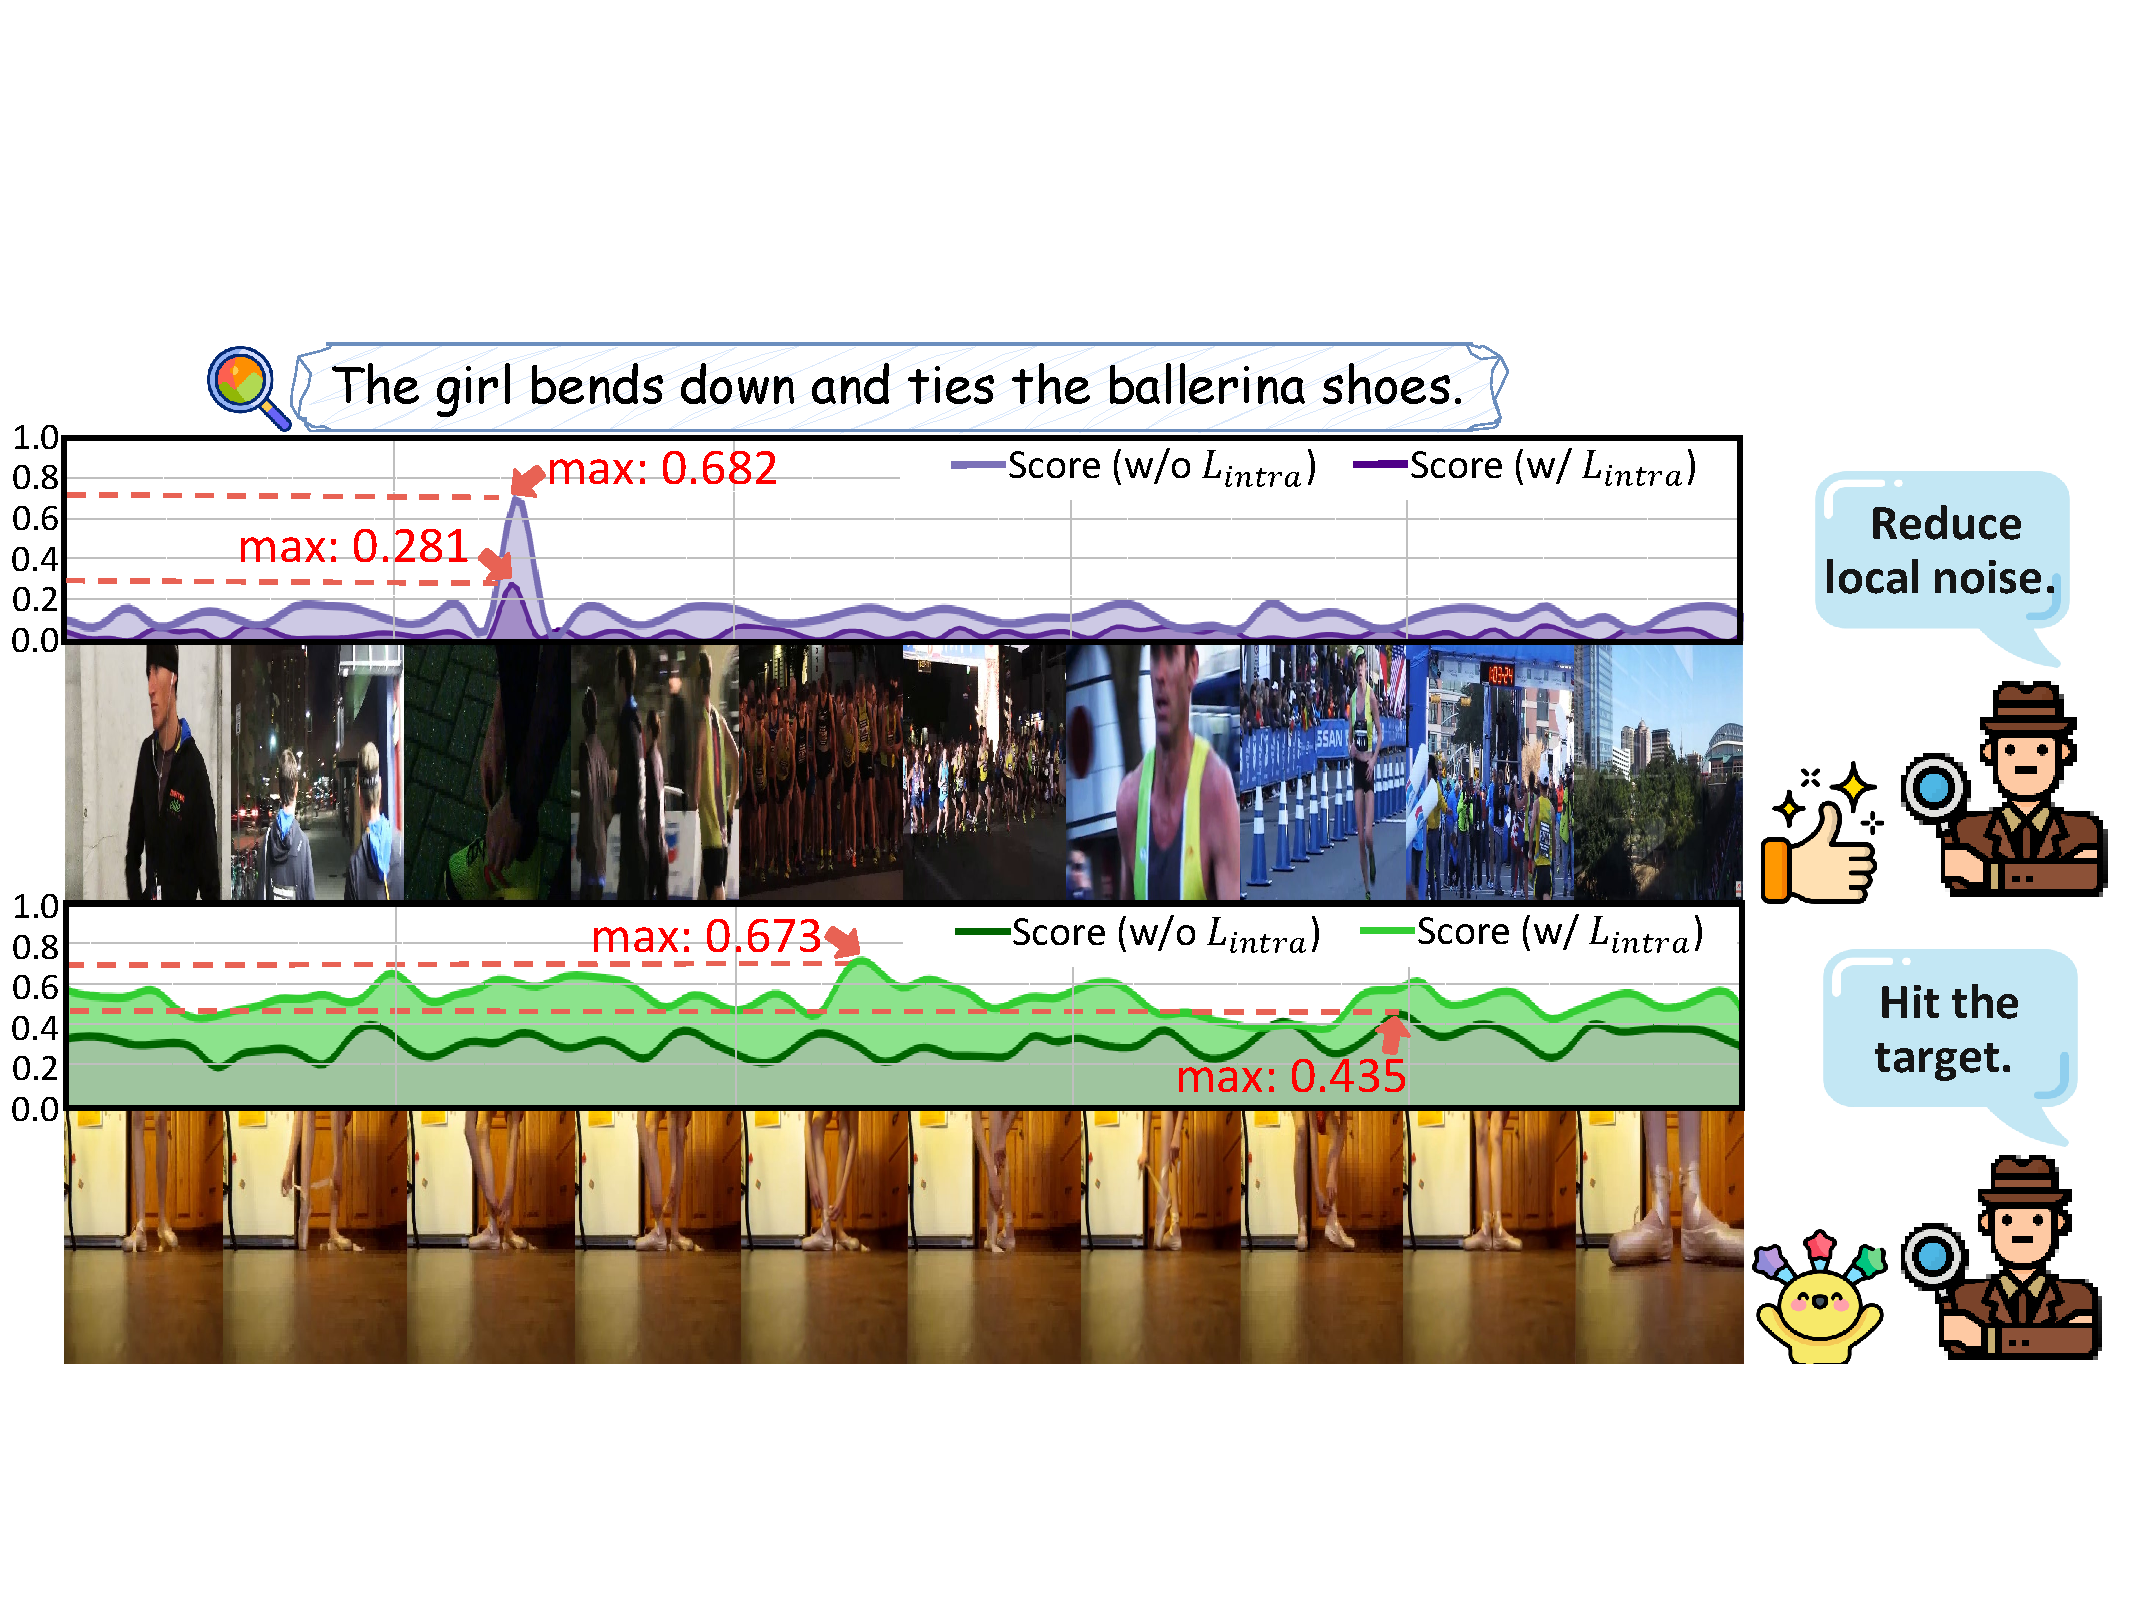
\includegraphics[width=\linewidth]{images/ablation_intra.pdf}
    \caption{使用\cref{fig:Intro} 中的同一组视频进行对比。移除 $L_{\mathrm{intra}}$ 后检索失败，无关视频得分高于真实匹配视频（0.682 对 0.435）。加入 $L_{\mathrm{intra}}$ 后，排序正确，真实匹配视频得分高于无关视频（无关视频为 0.281，真实匹配视频为 0.673）。}
    \label{fig:vis1}
    \vspace{-.3cm}
\end{figure}
\subsection{与先进方法对比}
\noindent \textbf{基线} \quad 我们选择 15 种有代表性的 PRVR 基线，并将 \modelname{} 与 T2VR 和 VCMR 方法进行比较。T2VR 对比方法包括 RIVRL\cite{dong2022reading}、CLIP4Clip\cite{luo2022clip4clip} 和 Cap4Video\cite{wu2023cap4video}。VCMR 对比方法包括 ReLoCLNet\cite{zhang2021video}、CONQUER\cite{hou2021conquer} 和 JSG\cite{jsg}。

\noindent \textbf{检索表现} \quad
\cref{tab:main} 汇总了各模型在三个基准上的检索表现。针对 PRVR 设计的方法整体优于 T2VR 和 VCMR 方法。\modelname{} 通过有效建模查询歧义、为更多视频片段提供可靠监督，达到了当前先进水平。具体而言，与最强竞争方法 DreamPRVR\cite{HLFormer} 相比，在 ActivityNet Captions 和 Charades-STA 上的 SumR 分别高 0.7 和 0.6。在 TVR 上，SumR 比 MGAKD\cite{MGAKD} 高 8.1。

\noindent \textbf{模型效率} \quad
\cref{tab:efficiency} 进一步比较了模型效率。所有结果为相同设置下 5 次运行的平均值。与规模相近的模型相比，\modelname{} 以相当的效率取得更好的性能，表明分层证据学习带来的开销很小。

\begin{figure}[t]
    \centering
    \parbox[b]{0.22\textwidth}{
        \centering
            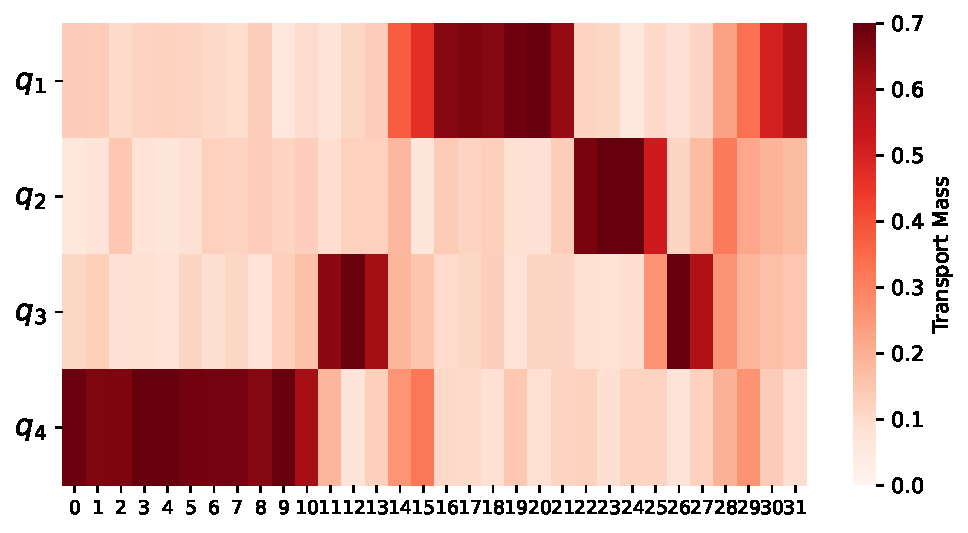
\includegraphics[width=\linewidth]{images/Standard_OT.pdf}
        \\[-0.45em]
        { \scalebox{0.85}{(a) 标准最优传输}}
    }
    \hspace{0.02\textwidth}
    \parbox[b]{0.22\textwidth}{
        \centering
            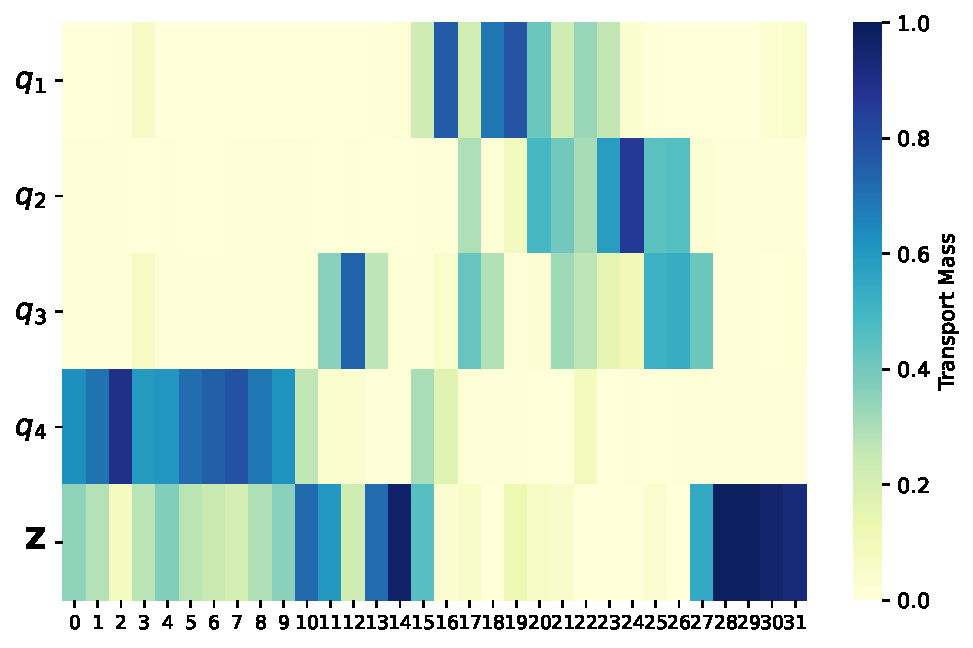
\includegraphics[width=\linewidth]{images/Flexible_OT.pdf}
        \\[-0.25em]
        {\scalebox{0.85}{(b) 灵活最优传输}}
    }
    \caption{OT 与 FOT 的传输质量对齐对比。$Z$ 表示回收槽。可视化结果显示，回收槽吸收了最后几个片段的传输质量。}
    \label{fig:pot}
\end{figure}
\subsection{模型分析}
\noindent \textbf{多尺度视频间证据学习} \quad
我们通过以下消融对多尺度分支进行评估：(i) 仅使用帧尺度或片段尺度分支，只用 $L^{f}_{U}$ 或 $L^{c}_{U}$ 训练；(ii) 移除动态协同证据聚合器，即训练时不使用 $L^{o}_{U}$。\cref{tab:ablation} 表明，单分支学习和移除聚合均会降低性能，说明多粒度视频间证据学习的必要性。结果还表明，跨分支证据聚合可提供整体不确定性估计，促进模型优化。

\noindent \textbf{划分融合策略的影响} \quad
我们比较三种策略：(i) 采信单一分支；(ii) 不确定性主导的划分融合（UDPF，默认），通过优先采信不确定性较高的类别处理分支冲突；(iii) 采用相反原则的置信度主导策略。\cref{tab:ablation} 表明，融合双分支预测可得到更可靠的划分并提高准确率。较为激进的置信度主导策略有时会产生过于自信却错误的关联，其性能低于较保守的 UDPF。

\noindent \textbf{查询标签校准的有效性} \quad
比较\cref{tab:ablation} 中编号 (0)、(8) 和 (9) 发现，未经校准的基线表现最差。我们认为，这是因为它忽略了固有的语义歧义，无差别地推远所有未配对视频，过度惩罚语义相关的样本，进而引入误导性监督。初步多义集合 $\tilde{\mathcal{S}}_n$ 又未能捕捉 $\tilde{\mathcal{S}}_p$ 中的多义查询，性能也非最优。这些结果进一步验证了对查询歧义建模和进行细粒度查询识别的重要性。


\noindent \textbf{视频内证据学习的有效性} \quad
\cref{tab:ablation} 中编号 (10) 的结果表明，移除 $L_{\mathrm{intra}}$ 会显著降低检索准确率。我们还在\cref{fig:vis1} 中可视化了查询与视频之间的时序注意力分数。加入 $L_{\mathrm{intra}}$ 后，模型降低了对无关视频的响应，减少了虚假局部尖峰，提高了相关视频的相似度分数。该目标通过一对多的软分配在查询和片段之间建立对应，汇聚多个相关片段的证据，从而提供更密集的时序监督，抑制虚假局部噪声，提高检索可靠性与准确率。


\noindent \textbf{灵活最优传输的作用} \quad
为了评估灵活最优传输的作用，我们比较三种变体：(i) 基于 softmax 的分配，(ii) 最优传输（OT），以及 (iii) 灵活最优传输（FOT，默认）。如\cref{tab:ablation} 所示，softmax 表现最差，OT 提升了性能，但无法捕捉 PRVR 中的部分相关性。如\cref{fig:pot} 所示，FOT 借助回收槽吸收噪声片段，减少由无关内容造成的错误对齐，因此表现最好。



\begin{figure}[t]
    \centering
        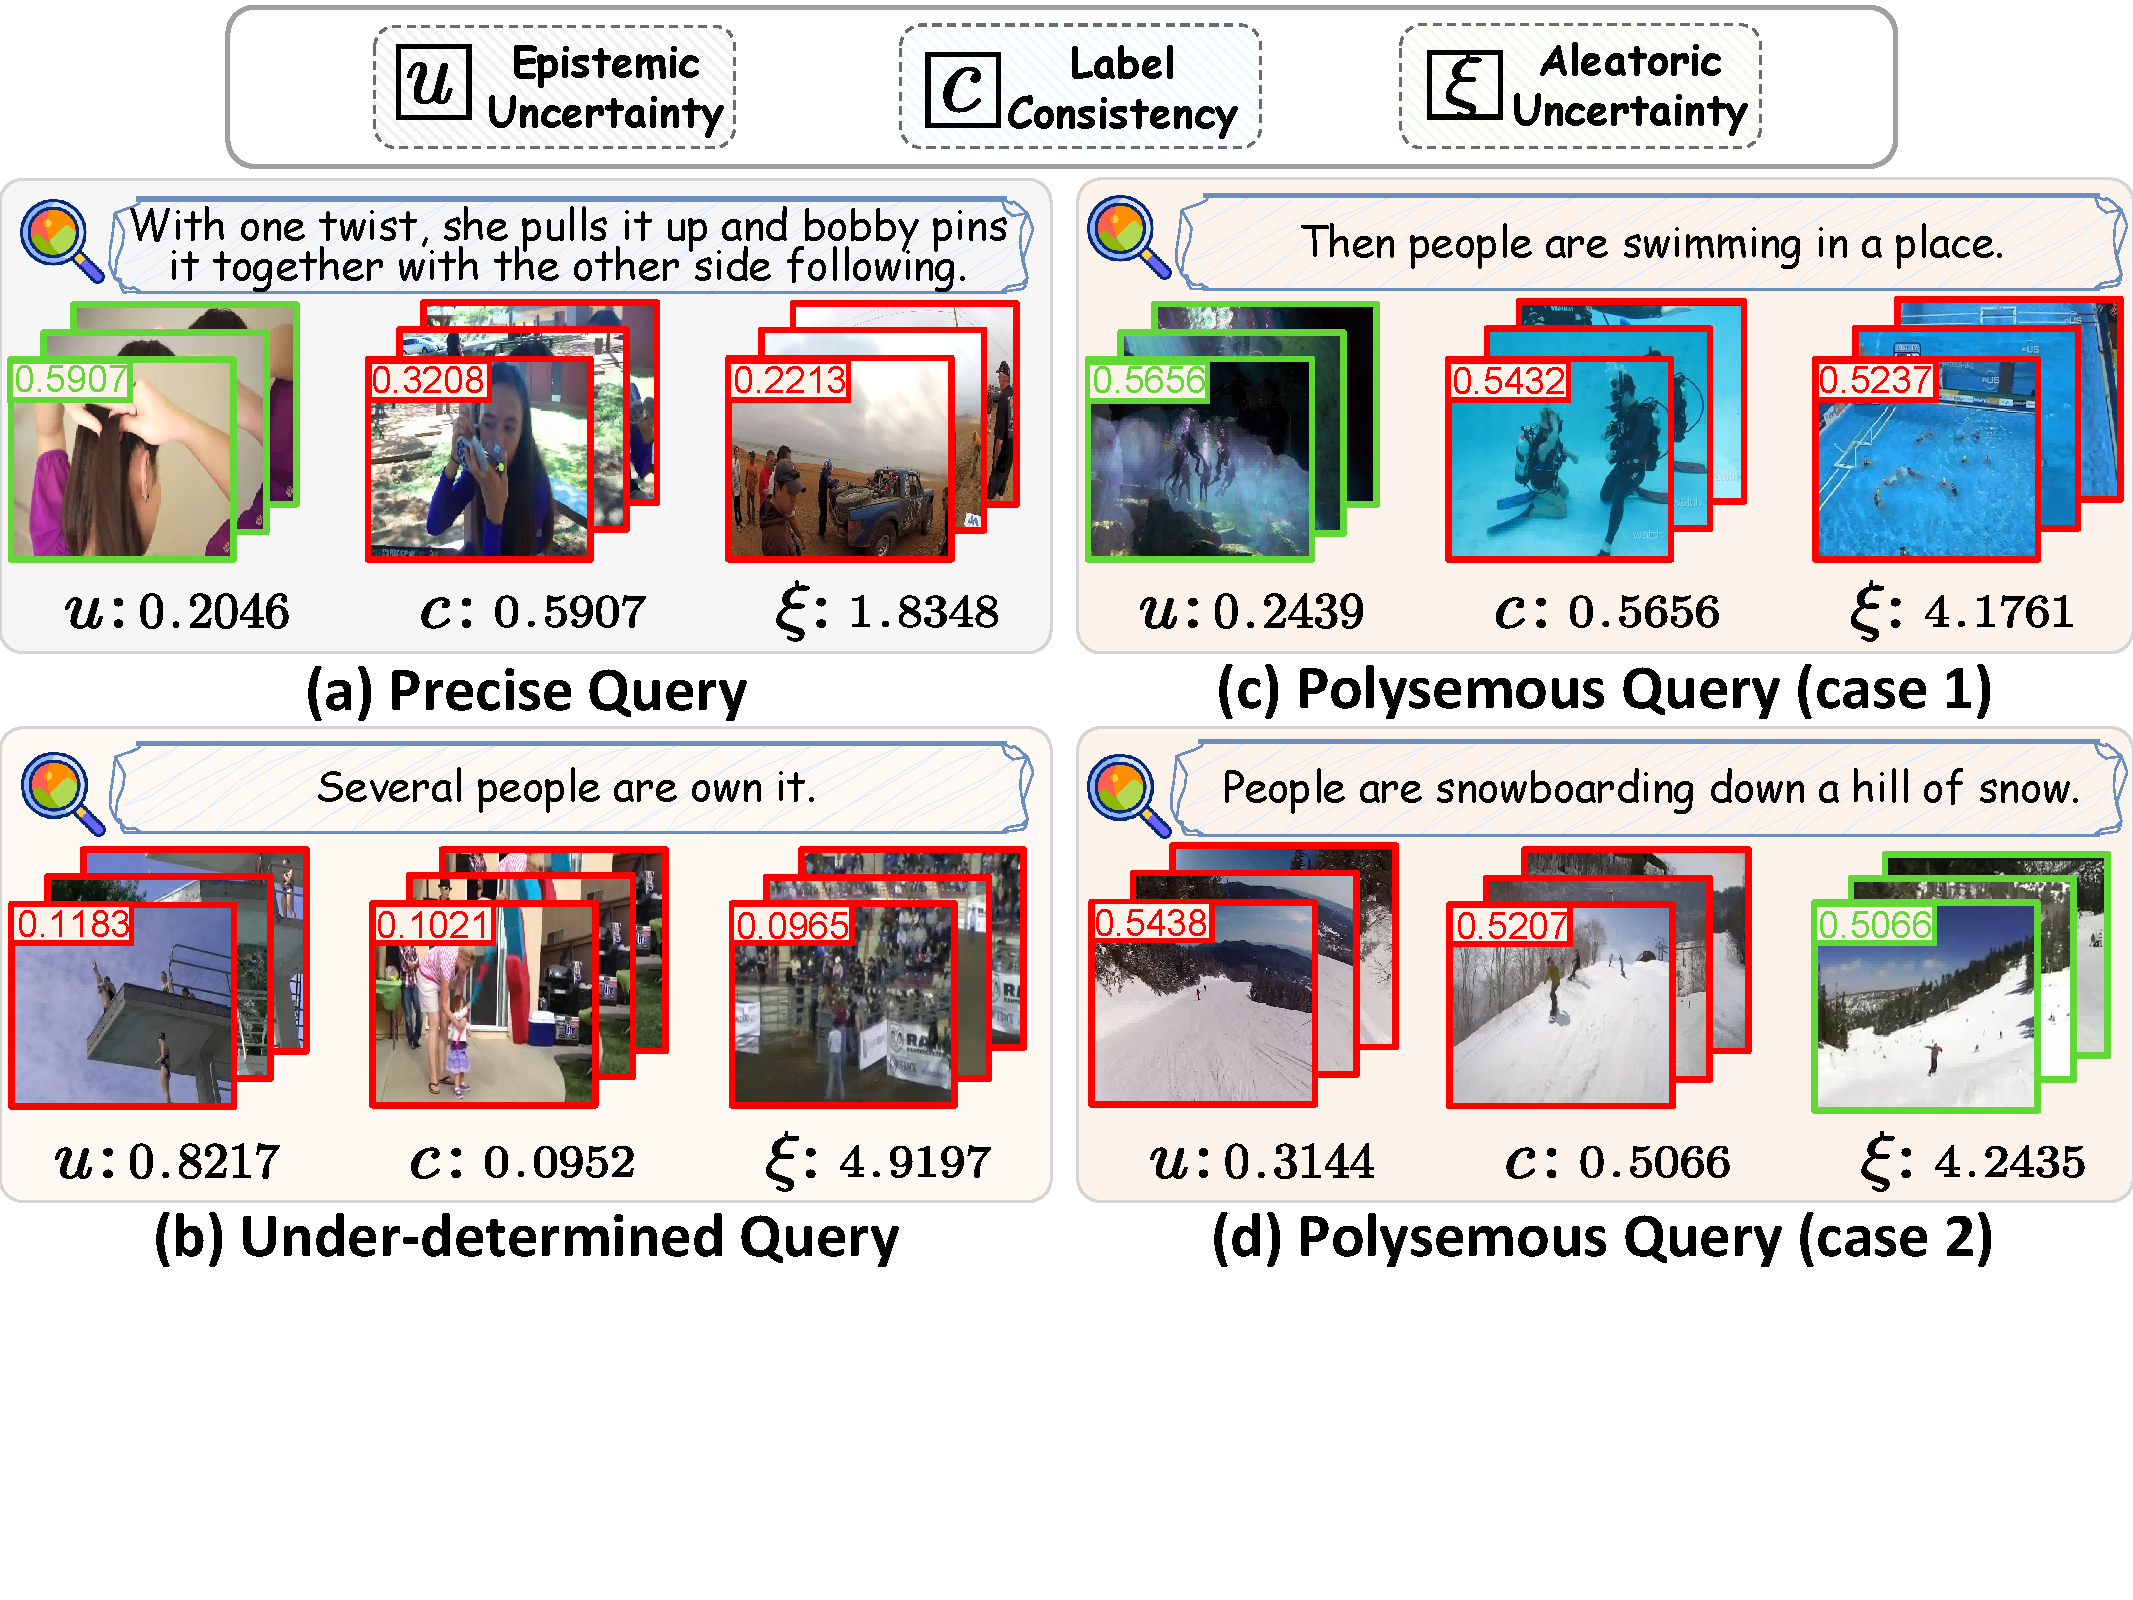
\includegraphics[width=0.48\textwidth]{images/query-choose.pdf}
    \caption{查询识别的定性示例。每条查询展示排名前三的视频，正确匹配用绿色边框标示，错误匹配用红色边框标示。每个视频的左上角显示相似度分数。}
    \label{fig:query-choose}
\end{figure}

\noindent \textbf{查询识别的定性结果} \quad
\cref{fig:query-choose} 展示了说明识别算法有效性的代表性示例。$u$ 与 $c$ 能清楚地分离信息不足查询，$\xi$ 则主要用于区分精确查询和多义查询，与我们的分类准则一致。我们观察到，相比缺乏明确指代线索且较短的多义查询，精确查询一般更长，也更具体。此外，信息不足查询可能含有语法或拼写错误（如误拼为 own），妨碍语义理解。这些观察符合实际场景，也进一步支持了本方法的有效性。

\section{结论}
\label{sec:conclusion}
本文提出了 \modelname{}，一种旨在处理 PRVR 内在不确定性和监督稀疏问题的分层证据学习框架。
为了处理视频间的查询歧义，\modelname{} 用 Dirichlet 分布将跨模态相似度建模为证据，按三项原则识别查询类型，并引导自适应的标签校准。
作为补充，我们在视频内引入带自适应回收槽的灵活最优传输，实现密集的时序对齐。该机制能在积累可靠监督信号的同时有效滤除噪声，从而提升检索性能。

\section*{局限性}
为公平比较，我们沿用既有工作，使用预训练模型（例如 ResNet）提取特征，这可能限制检索表现。未来计划采用更先进的编码器（例如 CLIP），并开展端到端训练。与多数检索方法一样，\modelname{} 需要访问完整视频，因而不太适合在线流式视频检索。

\section*{原论文致谢}
我们诚挚感谢审稿人和会议主席付出的努力以及提出的建设性意见，这些意见帮助我们改进了稿件。本研究获得国家自然科学基金项目（624B2088、62571298、62536003、62521006）以及鹏城实验室项目（PCL2025A14）的部分资助。

\section*{影响声明}
本文提出 PRVR 框架 \modelname{}，通过显式建模语义不确定性和查询歧义，提高人工智能系统的可靠性。除了提升检索准确率，这项工作的主要社会价值之一，是将确定性的“黑箱”预测转向可解释、能反映不确定性的检索。通过区分高置信匹配和证据不足的推测，我们的方法有助于提高下游应用的可信度，并为人工复核提供依据。先进的检索技术具有潜在的双重用途风险，例如可能用于自动监控。\modelname{} 通过视频内证据学习和自适应回收槽机制滤除虚假相关和噪声，主动减轻误报造成的危害。此外，通过显式区分多义查询和信息不足查询，该框架为诊断和分析数据集偏差提供了一种方法，从而减少对这些偏差的盲目过拟合。我们认为，重视不确定性量化和不可靠信号的抑制，有助于推动多模态视频理解朝着更稳健、透明和负责任的方向发展。


\section*{译者致谢}
感谢原作者公开论文、代码与复现实验资源。本中文译版以
\href{https://arxiv.org/abs/2605.06083v1}{arXiv:2605.06083v1} 为底本，
使用 Leey21 的 \href{https://github.com/Leey21/arxiv-translator}{arxiv-translator}
工作流制作。译文为非官方版本，按
\href{https://creativecommons.org/licenses/by/4.0/}{CC BY 4.0} 发布。

\bibliography{main}
\bibliographystyle{icml2026}

\newpage
\appendix
\onecolumn
\section{More Experiments}
\subsection{Hyper-Parameters} 
\label{hyperparameter}
We adopt the hyperparameter settings from HLFormer \cite{HLFormer} and GMMFormerV2 \cite{GMMFormerV2}. The numbers of clips and frames are set to $M_c=32$ and $M_f=128$, respectively. The maximum query length $N_q$ is fixed to 64 for ActivityNet Captions and 30 for TVR and Charades-STA. All remaining settings, including $L_{\text{sim}}$ and $L_{\text{div}}$, follow \cite{HLFormer}. Detailed implementation can be provided in the submitted code \href{https://github.com/lijun2005/ICML26-Holmes}{ICML26-Holmes}.


\subsection{Parameter Analysis}
We performed a comprehensive hyperparameter analysis on the TVR dataset to investigate the effects of the temperature $\tau$ in \cref{ea:evi1}, the threshold $\beta$ in \cref{eq:threshold}, and the dustbin bucket ratio $z$ in \cref{eq:new-s}, as depicted in \cref{fig:parameter_analysis}. The results indicate that our model maintains relatively stable performance when $\tau$ is within [0.06, 0.2], $\beta$ within [0.2, 0.5], and $z$ within [0.2, 0.4], demonstrating that the proposed approach is largely insensitive to hyperparameter variations and exhibits strong robustness.

\begin{figure*}[h]
    \centering
    \vspace{-0.8em}
    \parbox[b]{0.25\textwidth}{
        \centering
            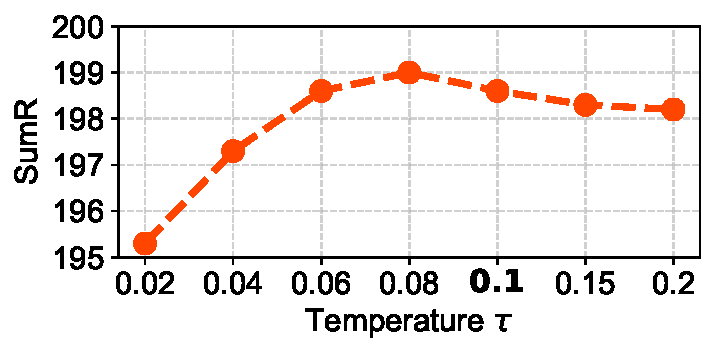
\includegraphics[width=\linewidth]{images/tvr_tau-.pdf}
    }
    \hspace{0.02\textwidth}
    \parbox[b]{0.25\textwidth}{
        \centering
            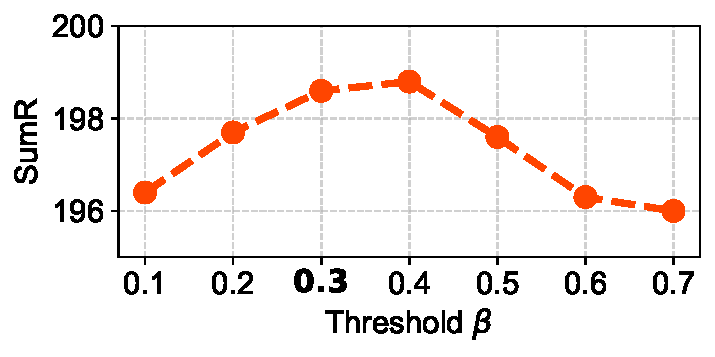
\includegraphics[width=\linewidth]{images/tvr_beta-.pdf}
    }
    \parbox[b]{0.25\textwidth}{
        \centering
            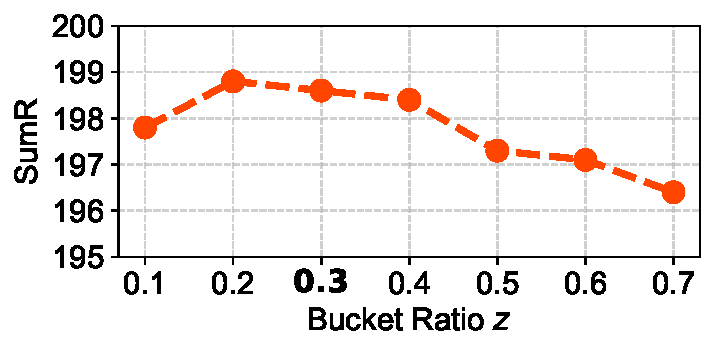
\includegraphics[width=\linewidth]{images/tvr_ratio-.pdf}
    }
    \hspace{0.02\textwidth}
    \vspace{-0.6em}
    \caption{The parameter analysis of the temperature $\tau$ in \cref{ea:evi1}, the threshold $\beta$ in \cref{eq:threshold}, and the dustbin bucket ratio $z$ in \cref{eq:new-s} on the TVR dataset, with the default settings highlighted in bold.
    }
    \label{fig:parameter_analysis}
\end{figure*}
\section{More Details on Method}
\subsection{Basic Training Objectives}
 Following  existing works\cite{ms-sl,GMMFORMER}, we adopt triplet loss \cite{dong2021dual, faghri2017vse++} $L^{trip}$ and InfoNCE loss \cite{miech2020end, zhang2021video} $L^{nce}$, query diverse loss \cite{GMMFORMER} $L_{div}$ that are widely used in PRVR. A text-video pair is considered positive if the video contains a moment relevant to the text; otherwise, it is regarded as negative.
 Given a positive text-video pair $({T}, {V})$, the triplet ranking loss over the mini-batch $\mathcal{B}$ is formulated as:
\begin{gather}
L^{trip} = \frac{1}{n} \sum_{({T},{V}) \in {B}} \{\text{max}(0, m + s({T}^-, {V}) - s({T}, {V})) \nonumber 
    + \text{max}(0, m + s({T}, {V}^-) - s({T},{V}))\},
\end{gather}
where $m$ is a margin constant. ${T}^-$ and ${V}^-$ indicate a negative text for ${V}$ and a negative video for ${T}$, respectively. The similarity score $s(,)$ is obtained by \cref{eq:simscore} and \cref{eq:sim}.

 The infoNCE loss  is computed as:
\begin{gather}
L^{nce} = -\frac{1}{n} \sum_{({T},{V}) \in \mathcal{B}} \left\{\text{log}\left(\frac{s({T},{V})}{s({T},{V}) + \sum\nolimits_{{T}_i^{-} \in \mathcal{N}_{T} }s({T}_i^-, {V})}\right) \nonumber
+ \text{log}\left(\frac{s({T},{V})}{s({T},{V}) + \sum\nolimits_{{V}_i^{-} \in \mathcal{N}_{V} }s({T}, {V}_i^-)}\right) \right\},
\end{gather}
where $ \mathcal{N}_{T} $ and $ \mathcal{N}_{V} $ represent the negative texts and videos of $ {V} $ and $ {T} $ within the mini-batch $ \mathcal{B} $, respectively.

Finally , $L_{sim}$ is defined as:
\begin{equation}
L_{sim} = L_{c}^{trip} + L_{f}^{trip} + \lambda_c L_{c}^{nce} + \lambda_f L_{f}^{nce},
\end{equation}
where  $f$ and $c$ mark the objectives for the frame-level branch and the  clip-level branch, respectively.
 $\lambda_c$ and $\lambda_f$ are hyper-parameters to balance the contributions of InfoNCE objectives.


Given a collection of text queries $T$ in the mini-batch $\mathcal{B}$, the query diverse loss is defined as:
\vspace{-.5em}
\begin{equation}
L_{div} = \frac{1}{n} \sum_{\boldsymbol q_i,\boldsymbol q_j \in {T}} \mathds{1}_{\boldsymbol q_i, \boldsymbol q_j} \log\left(1 + e^{\alpha (cos(\boldsymbol q_i, \boldsymbol q_j) + \delta)}\right),
\vspace{-.5em}
\end{equation}
where $ \delta > 0 $ denotes the margin, $ \alpha > 0 $ is a scaling factor, and $ \mathds{1}_{\boldsymbol q_i, \boldsymbol q_j} \in \{0,1\} $ represents an indicator function,  $ \mathds{1}_{\boldsymbol q_i, \boldsymbol q_j} = 1 $ when  $ \boldsymbol q_i $ and $ \boldsymbol q_j $ correspond to the same video.
\subsection{Detailed proofs for \cref{theorem: wrong uncertainty}}
\label{appendix:theorem3.2}

\begin{proof}
We prove the theorem by providing a counter-example.
Let $y_i$ be the ground-truth label corresponding to index $t$ (i.e., $y_{it}=1$).
Let $\boldsymbol{e}_i$ be an evidence vector constructed such that all evidence is assigned to an incorrect video $k$ ($k \neq t$):
\begin{equation}
    e_{ij} = 
    \begin{cases}
    \lambda, & \text{if } j = k, \\
    0, & \text{otherwise},
    \end{cases}
\end{equation}
where $\lambda \gg 0$ is a large positive constant.
According to Eq. (\ref{eq:dir-alpha}) and Eq. (\ref{eq:dir-alpha2}), the Dirichlet strength is $S_i = \lambda + K$.
Consequently, the epistemic uncertainty is $\displaystyle u_i = \frac{K}{\lambda + K}$. By choosing a sufficiently large $\lambda$, we can make $u_i$ arbitrarily close to 0 (low uncertainty).

However, the belief mass $b_{ij}$ is maximized at index $k$ because $\alpha_{ik} > \alpha_{ij}$ for all $j \neq k$.
Since $k \neq t$, the highest belief is not assigned to the annotated label.
This implies that a low epistemic uncertainty indicates that the model has collected a large amount of evidence, but it does not guarantee that this evidence points to the correct video.
\end{proof}

\subsection{The derivation of aleatoric uncertainty in \cref{eq:aleatoric-uncertainty}}
\label{appendix:aleatoric-uncertainty}
Following standard formulations in evidential learning \citep{rule, r-edl}, let $\mathbf{p} = [p_1, \dots, p_K]^\top$ be the probability vector for the $i$-th sample, defined on the $K$-dimensional unit simplex $\mathcal{S}^K$. We assume $\mathbf{p}$ follows a Dirichlet distribution parameterized by the concentration vector $\boldsymbol{\alpha}_i = [\alpha_{i1}, \dots, \alpha_{iK}]^\top$. The probability density function (PDF) is defined as:
\begin{equation}
    \text{Dir}(\mathbf{p}; \boldsymbol{\alpha}_i) = 
    \begin{cases} 
        \displaystyle\frac{1}{B(\boldsymbol{\alpha}_i)} \prod_{k=1}^{K} p_k^{\alpha_{ik}-1}, & \text{for } \mathbf{p} \in \mathcal{S}^K, \\
        0, & \text{otherwise},
    \end{cases}
    \label{eq:dirichlet_pdf}
\end{equation}
where $B(\boldsymbol{\alpha}_i) = \frac{\prod_{k=1}^K \Gamma(\alpha_{ik})}{\Gamma(S_i)}$ is the multivariate beta function, and $S_i = \sum_{k=1}^K \alpha_{ik}$ is the strength of the distribution. The expected entropy (aleatoric uncertainty) of the random variable $\mathbf{p}$ under this distribution is derived as follows:
\begin{equation}
\begin{split}
\mathbb{E}_{\mathbf{p} \sim \text{Dir}(\boldsymbol{\alpha}_i)} [H(\mathbf{p})] 
    &= \int_{\mathcal{S}^K} \text{Dir}(\mathbf{p}; \boldsymbol{\alpha}_i) \left( - \sum_{k=1}^{K} p_k \ln p_k \right) d\mathbf{p} \nonumber \\
    &= - \sum_{k=1}^{K} \int_{\mathcal{S}^K} \text{Dir}(\mathbf{p}; \boldsymbol{\alpha}_i) (p_k \ln p_k) d\mathbf{p} \nonumber \\
    &= - \sum_{k=1}^{K} \int_{\mathcal{S}^K} \frac{\Gamma(S_i)}{\prod_{j=1}^{K} \Gamma(\alpha_{ij})} \prod_{j=1}^{K} p_j^{\alpha_{ij}-1} (p_k \ln p_k) d\mathbf{p} \nonumber \\
    &= - \sum_{k=1}^{K} \int_{\mathcal{S}^K} \frac{\alpha_{ik}}{S_i} \frac{\Gamma(S_i + 1)}{\Gamma(\alpha_{ik} + 1) \prod_{j \neq k} \Gamma(\alpha_{ij})} p_k^{\alpha_{ik}} \prod_{j \neq k} p_j^{\alpha_{ij}-1} \ln p_k d\mathbf{p} \nonumber \\
    &= - \sum_{k=1}^{K} \frac{\alpha_{ik}}{S_i} \int_{\mathcal{S}^K} \text{Dir}(\mathbf{p}; \boldsymbol{\alpha}_i + \mathbf{1}_k) \ln p_k d\mathbf{p} \nonumber \\
    &= - \sum_{k=1}^{K} \frac{\alpha_{ik}}{S_i} \mathbb{E}_{\mathbf{p} \sim \text{Dir}(\boldsymbol{\alpha}_i + \mathbf{1}_k)} [\ln p_k] \nonumber \\
    &= - \sum_{k=1}^{K} \frac{\alpha_{ik}}{S_i} (\psi(\alpha_{ik} + 1) - \psi(S_i + 1)) \nonumber \\
    &= \sum_{k=1}^{K} \frac{\alpha_{ik}}{S_i} (\psi(S_i + 1) - \psi(\alpha_{ik} + 1)),
\end{split}
\end{equation}
where the term $\mathbf{1}_k$ represents a one-hot vector with the $k$-th element set to 1 and all others set to 0. The derivation primarily relies on the recursive property of the Gamma function, $\Gamma(z+1) = z\Gamma(z)$. This property allows us to rewrite the probability density function by extracting the factor $\displaystyle\frac{\alpha_{ik}}{S_i}$, thereby transforming the original integral into an expectation over a new Dirichlet distribution with parameters shifted by $\mathbf{1}_k$ (i.e., $\boldsymbol{\alpha}_i + \mathbf{1}_k$).
\subsection{The derivation of loss function in \cref{eq:evi-loss}}
\label{appendix:equation17}
In this section, we provide the detailed derivation of the evidential learning objective presented in the main paper. 

Our method aims to guide the predicted probability $\boldsymbol{p}_i$ to align with the calibrated label $\hat{\boldsymbol{y}}_i$. Since $\boldsymbol{p}_i$ is a random variable, we formulate the uncertainty-aware learning objective as the expected sum of squared errors between $\hat{\boldsymbol{y}}_i$ and $\boldsymbol{p}_i$. The derivation is as follows:
\begin{equation}
\setlength{\abovedisplayskip}{2pt}
\setlength{\belowdisplayskip}{2pt}
    \begin{split}
        {L}_U(\boldsymbol{\alpha}_i, \hat{\boldsymbol{y}}_i)
        &=\int\left\|\hat{\boldsymbol y}_i-\boldsymbol{p}_i\right\|_2^2 \frac{1}{B\left(\boldsymbol{\alpha}_i\right)} \prod_{j=1}^{K} p_{i j}^{\alpha_{i j}-1} d \boldsymbol{p}_i \\
        &= \int \|\hat{\boldsymbol{y}}_i - \boldsymbol{p}_i\|_2^2 \, \text{Dir}(\boldsymbol{p}_i; \boldsymbol{\alpha}_i) \, d\boldsymbol{p}_i \\
        &= \sum_{j=1}^K \mathbb{E}_{\boldsymbol{p}_i \sim \text{Dir}(\boldsymbol{\alpha}_i)} \left[ (\hat{y}_{ij} - p_{ij})^2 \right] \\
        &= \sum_{j=1}^K \left[ \left( \hat{y}_{ij} - \mathbb{E}[p_{ij}] \right)^2 + \text{Var}(p_{ij}) \right] \\
        &= \sum_{j=1}^K \left( \hat{y}_{ij} - \frac{\alpha_{ij}}{S_i} \right)^2 + \frac{\alpha_{ij} (S_i - \alpha_{ij})}{S_i^2 (S_i + 1)},
    \end{split}
\end{equation}
where $S_i = \sum_{j=1}^K \alpha_{ij}$. The third step utilizes the standard bias-variance decomposition, $\mathbb{E}[(X-c)^2] = (c-\mathbb{E}[X])^2 + \text{Var}(X)$, and the final step substitutes the mean and variance of the Dirichlet distribution: $\mathbb{E}[p_{ij}] = \alpha_{ij}/S_i$ and $\text{Var}(p_{ij}) = \alpha_{ij}(S_i-\alpha_{ij}) / [S_i^2(S_i+1)]$.
\subsection{Derivation of the Sinkhorn Algorithm}
\label{sec:sinkhorn_derivation}
In this section, we provide a detailed derivation of the Sinkhorn algorithm used for calculating the optimal transport (\cref{eq:ot}). 
Consider a similarity matrix $\mathbf{S} \in \mathbb{R}^{n \times m}$, where $[\mathbf{S}]_{i,j}$ represents the similarity score between a video clip $\mathbf{c}_i$ and a query $\mathbf{q}_j$. The goal of optimal transport is to find a transport plan $\mathbf{Q}$ that maximizes the total similarity under marginal constraints. The primal problem is defined as:
\begin{equation}
\begin{aligned}
    \max_{\mathbf{Q} \in \mathcal{Q}} \quad & \langle \mathbf{Q}, \mathbf{S} \rangle = \text{tr}(\mathbf{Q}^\top \mathbf{S}) = \sum_{i=1}^{n} \sum_{j=1}^{m} [\mathbf{Q}]_{i,j} \cdot [\mathbf{S}]_{i,j} \\
    \text{s.t.} \quad & \mathcal{Q} = \left\{ \mathbf{Q} \in \mathbb{R}_+^{n \times m} \mid \mathbf{Q}\mathbf{1}_m = \boldsymbol{\mu}, \, \mathbf{Q}^\top \mathbf{1}_n = \boldsymbol{\nu} \right\},
\end{aligned}
\label{eq:ot_primal}
\end{equation}
where $\boldsymbol{\mu} \in \mathbb{R}^n$ and $\boldsymbol{\nu} \in \mathbb{R}^m$ are probability vectors representing the mass distribution of video clips and queries, respectively. For uniform distributions, we set $\boldsymbol{\mu} = \frac{1}{n}\mathbf{1}_n$ and $\boldsymbol{\nu} = \frac{1}{m}\mathbf{1}_m$.

Standard linear programming solvers for Eq.~\eqref{eq:ot_primal} typically require $O(n^3 \log n)$ time complexity, which is computationally prohibitive for large-scale datasets. To address this, Cuturi \citep{sinkhorn} proposed an entropy-regularized formulation that admits a fast approximate solution:
\begin{equation}
    \max_{\mathbf{Q} \in \mathcal{Q}} \quad \langle \mathbf{Q}, \mathbf{S} \rangle + \varepsilon H(\mathbf{Q}),
    \label{eq:ot_regularized}
\end{equation}
where $H(\mathbf{Q}) = - \sum_{i,j} [\mathbf{Q}]_{i,j} \ln([\mathbf{Q}]_{i,j})$ is the entropy regularization term and $\varepsilon > 0$ is the regularization coefficient. This convex objective function allows us to utilize the Lagrange multiplier method. The Lagrangian $\mathcal{L}(\mathbf{Q}, \boldsymbol{u}, \boldsymbol{v})$ with dual multipliers $\boldsymbol{u} \in \mathbb{R}^n$ and $\boldsymbol{v} \in \mathbb{R}^m$ is given by:
\begin{equation}
    \mathcal{L}(\mathbf{Q}, \boldsymbol{u}, \boldsymbol{v}) = \langle \mathbf{Q}, \mathbf{S} \rangle + \varepsilon H(\mathbf{Q}) + \boldsymbol{u}^\top (\mathbf{Q}\mathbf{1}_m - \boldsymbol{\mu}) + \boldsymbol{v}^\top (\mathbf{Q}^\top \mathbf{1}_n - \boldsymbol{\nu}).
    \label{eq:lagrangian}
\end{equation}
Taking the partial derivative of Eq.~\eqref{eq:lagrangian} with respect to each entry $[\mathbf{Q}]_{i,j}$ and setting it to zero (KKT condition):
\begin{equation}
    \frac{\partial \mathcal{L}}{\partial [\mathbf{Q}]_{i,j}} = [\mathbf{S}]_{i,j} - \varepsilon (\ln([\mathbf{Q}]_{i,j}) + 1) + u_i + v_j = 0.
\end{equation}
Solving for $[\mathbf{Q}]_{i,j}$, we obtain:
\begin{equation}
    [\mathbf{Q}]_{i,j} = \exp\left( \frac{[\mathbf{S}]_{i,j} + u_i + v_j}{\varepsilon} - 1 \right) = e^{-\frac{1}{2} + \frac{u_i}{\varepsilon}} \cdot e^{\frac{[\mathbf{S}]_{i,j}}{\varepsilon}} \cdot e^{-\frac{1}{2} + \frac{v_j}{\varepsilon}}.
\end{equation}
This factorization suggests that the optimal solution $\mathbf{Q}^*$ can be expressed in terms of two scaling vectors, $\boldsymbol{\kappa}_1 \in \mathbb{R}^n$ and $\boldsymbol{\kappa}_2 \in \mathbb{R}^m$. By defining $\displaystyle[\boldsymbol{\kappa}_1]_i = \exp\left(-{1}/{2} + {u_i}/{\varepsilon}\right)$ and $\displaystyle[\boldsymbol{\kappa}_2]_j = \exp\left(-{1}/{2} + {v_j}/{\varepsilon}\right)$, the optimal transport matrix takes the form of a normalized exponential matrix:
\begin{equation}
    \mathbf{Q}^* = \text{Diag}(\boldsymbol{\kappa}_1) \exp(\mathbf{S}/\varepsilon) \text{Diag}(\boldsymbol{\kappa}_2).
    \label{eq:optimal_Q}
\end{equation}
Since $\mathbf{Q}^*$ must satisfy the marginal constraints in Eq.~\eqref{eq:ot_primal}, we have:
\begin{equation}
    \mathbf{Q}^*\mathbf{1}_m = \boldsymbol{\mu} \quad \text{and} \quad \mathbf{Q}^{*\top}\mathbf{1}_n = \boldsymbol{\nu}.
\end{equation}
Substituting Eq.~\eqref{eq:optimal_Q} into these constraints leads to the Sinkhorn-Knopp fixed-point iteration updates:
\begin{equation}
    \boldsymbol{\kappa}_1 \leftarrow \boldsymbol{\mu} \oslash (\exp(\mathbf{S}/\varepsilon) \boldsymbol{\kappa}_2), \quad 
    \boldsymbol{\kappa}_2 \leftarrow \boldsymbol{\nu} \oslash (\exp(\mathbf{S}^\top/\varepsilon) \boldsymbol{\kappa}_1),
\end{equation}
where $\oslash$ denotes element-wise division. Empirically, a few iterations (e.g., 50 steps) are sufficient to converge to a satisfactory transport plan $\mathbf{Q}^*$. The final optimal transport distance is then computed as $\langle \mathbf{Q}^*, \mathbf{S} \rangle$.
\subsection{Further details of Our Architecture}
We replace the standard self-attention in the Transformer block with Gaussian attention \cite{GMMFORMER}, yielding a Gaussian block.
Multiple Gaussian blocks ($N_g$) operate in parallel, and their outputs are aggregated via MAIM \cite{HLFormer} to construct the frame-/clip-level encoder.
For notational convenience, we unify the frame and clip embeddings as $\bmV_o$, since they are processed in an identical manner.
Given $\bmV_o$, the Gaussian attention is defined as:
\vspace{-.6em}
\begin{equation}\label{eq:euclidean-attention}
  \!\! \!\! \text{GA}({\bmV_o})\! =\!\text{softmax}\!\left(\!\mathcal{M}_{\sigma}^{g} \odot \frac{ {\bmV_o} W^q ( {\bmV_o} W^k)^{\top}}{\sqrt{d_h}}\!\right)\!{\bmV_o} W^v,
\vspace{-.6em}
\end{equation}
where $\displaystyle\mathcal{M}_{\sigma}^{g}(i, j) = \frac{1}{2\pi} e^{-\frac{(j-i)^2}{\sigma^2}}$ is a Gaussian kernel with variance $\sigma^2$. Varying $\sigma$ enables modeling feature interactions at different temporal scales, yielding multi-receptive-field representations. $W^q$, $W^k$ and $W^v$ denote linear projections. $d_h$ is the attention dimension and $\odot$ indicates element-wise multiplication.
\subsection{Further discussion  of related work}
Existing evidential learning methods have been applied to noisy cross‑modal retrieval and text‑to‑video retrieval, In noisy settings, prior works\cite{decl,ucpm} leverage epistemic uncertainty derived from Dirichlet parameters to identify instance-level noisy pairs (i.e., clean vs. noisy). In text-video retrieval, ~\cite{duq} integrates probabilistic embeddings with epistemic uncertainty only as a regularization signal. They do not explicitly model query-level semantic heterogeneity and also fail to address the unique challenges of PRVR.

Holmes introduces a hierarchical evidential framework specifically designed for PRVR:
\begin{itemize}
    \item Inter-video: PRVR queries exhibit fine-grained heterogeneity beyond a simple clean/noisy dichotomy. We propose a three-fold principle that goes beyond epistemic uncertainty by incorporating label consistency and aleatoric uncertainty for query diagnosis, enabling cross-scale conflict-aware fusion and query-adaptive label calibration.
    \item  Intra-video: PRVR relies on MIL to handle partial relevance, which induces sparse supervision. We employ FOT to provide denser supervision, generating reliable intra‑video evidence to support inter‑video learning.
\end{itemize}



\end{document}
